\chapter{VANS macroscopic applications}

\chapquote{The first principle is that you must not fool yourself — and you are the easiest person to fool.}{1974 Caltech commencement address}{Richard Feynman}

\section{Introduction}

In this chapter the macroscopic VANS equations are validated against a full microscopic DNS. Special attention is focused on the interface treatment using the penalization method. We also assess the effects of the permeability tensor metamodel within the algorithm. Computations are performed initially on the classical closed cavity configuration. The aim for the cavity problem is to validate the VANS approach and show the importance of the interface treatment and the permeability metamodel. In the last part the Ercoftac periodic hill case is also tested. This open configuration aims to test the performance of porous coating as a device to reduce separated flow.


\section{Closed cavity problem}
The configuration chosen is the square closed cavity, depicted in figure \ref{fig:geom}.
The cavity is square shaped with size $L$, the lateral and bottom walls are fixed and a constant velocity $U^{top}$ is specified at the top side.
On the front and back side we apply periodic boundary conditions since the simulation domain has a depth equal to $\ell$.
A rigid porous medium made by regularly arranged fibers is set at the bottom of the cavity, its vertical extension is equal to $h$.
The \textit{reference elementary volume} (REV) of the porous medium is a cubic cell of size $\ell$ with a cylinder, with diameter $d$, at its center.
The porosity of the medium, $\varepsilon$, is equal to 0.8 and 50 fibers are assumed to be present in the cavity.

\begin{figure}[h]
\centering
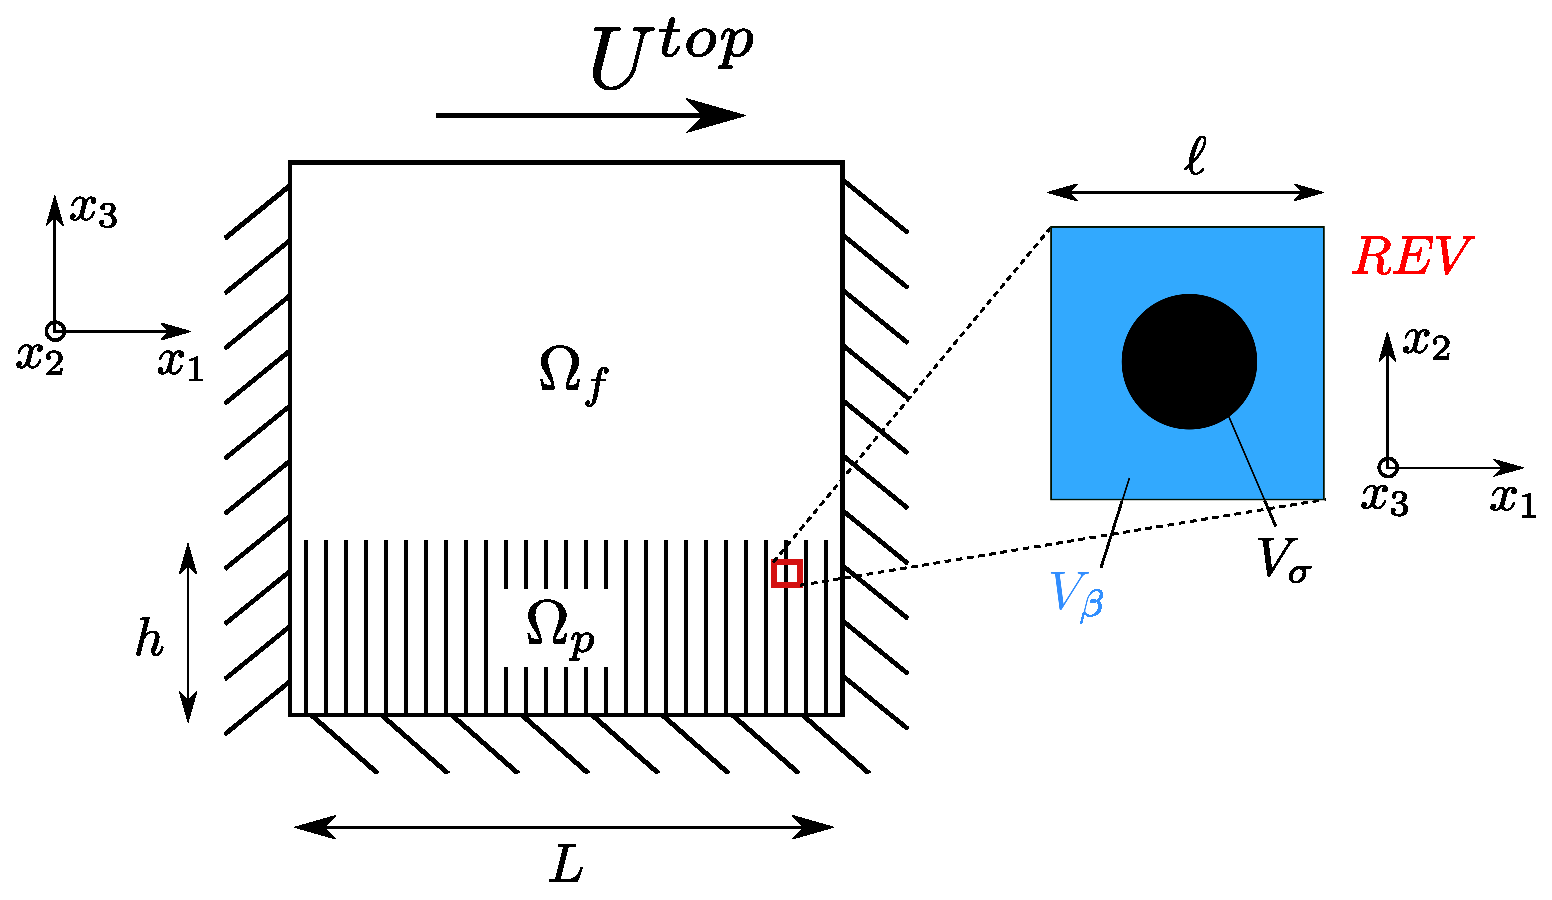
\includegraphics[width=0.7\linewidth]{chapter_5/figure/cavity_draw.eps}
\caption{Schematics of the closed cavity 2D problem. The porous medium internal structure is depicted in the zoom on the right side in which the REV geometry is shown.}
\label{fig:geom}
\end{figure}

To summarize the configuration:
\begin{itemize}
	\item $L$: side of the cavity, also the macroscopic length scale
	\item $h$: vertical extension of the fibers from the bottom of the cavity 
	\item $\ell$: side of the cubic REV, also the microscopic length scale
	\item $d$: diameter of the cylindrical fiber
	\item $V_{\beta}$: volume of the fluid inside the REV
	\item $V_{\sigma}$: volume of the solid inside the REV
	\item $\varepsilon = \dfrac{V_{\beta}}{V_{\sigma} +V_{\beta}} = \dfrac{\ell^3 -\ell \pi d^2 / 4}{\ell^3} = 1 - \pi \left(\dfrac{d}{2 \ell}\right)^2$: porosity of the medium
	\item $\epsilon = \dfrac{\ell}{L}$: length scale ratio
	\item $Re= \dfrac{U^{top} L}{\nub}$: Reynolds number of the cavity
\end{itemize}

The overall domain has the size $L \, \times \, L \times \, \ell$ respectively in the $x_1$, $x_2$ and $x_3$ directions. The origin of our coordinate system at the bottom left corner of the cavity. 
This configuration and porous arrangement has been chosen to employ DNS data already available for this configuration (private communication with \citet{zampogna2016fluid}).

The length parameters for the specific case are:
\begin{itemize}
	\item $h/L=0.33$
	\item $\ell/L=0.02$
	\item $\varepsilon = 0.8$
\end{itemize}

\subsection{Microscopic approach with direct numerical simulations}

In this approach the incompressible Navier-Stokes equations are solved in the three dimensional case \eqref{eq:NScavity}. 
The problem is weakly three dimensional since we include only one REV along the $x_3$ axes and we impose periodic boundary condition in this direction.
This assumption seems fair since the Reynolds numbers tested are small and no 3D structures are expected in the flow.
To complete the set of boundary conditions the no-slip condition is applied at the rigid walls and a prescribed horizontal velocity is imposed at the top wall \eqref{eq:NScavity}. The subscript $\beta$ means that the variables belongs to the fluid phase, as usual. The mesh is fine enough to resolve the flow within the fibers and the spatial converged is also assured.

% (50000 hexahedral cells including a refinement at the interface)

\begin{eqnarray}
\begin{cases}
\derp{\vb}{t} + \vb \cdot \nabla \vb = -\frac{1}{\rho_{\beta}} \nabla \pb + \nub \nabla^2  \vb \\
\nabla \cdot \vb = 0\\
\vb = 0 \qquad \text{on} \quad x_1 = 0,L \quad x_2 = 0 \\
\vb = U^{top} \qquad \text{on} \quad x_2 = L\\
\vb|_{x_3 = 0} = \vb|_{x_3 = \ell}  \\
\pb|_{x_3 = 0} = \pb|_{x_3 = \ell}
\end{cases}
\label{eq:NScavity}
\end{eqnarray}

Once the system \eqref{eq:NScavity} is solved, the microscopic fields (velocity and pressure) inside the porous medium are averaged with the operator \ref{eq:supavg} in order to get the homogenized macroscopic field $\meani{\vb}$ and $\meani{\pb}$.

\begin{equation}
	\meani{\psi_{\beta}} = \dfrac{1}{\volb} \int_{\volb} \psi_\beta (\mathbf{x}) d \volb.
	\label{eq:supavg}
\end{equation}

The operator \eqref{eq:supavg} has been applied through the whole porous domain using a REV with dimension $\ell \times \ell \times \ell$.
It means that the centroid of the REV, in which the average operation is performed, spans all the porous domain extension.
It should be noted that the averaging procedure gives a two dimensional averaged field as a result, the only not zero values are in the $x_1$ and $x_2$ directions. This is due to the symmetry of velocity and pressure in the $x_3$ direction that return zero averaged field as a result of the averaging operation \eqref{eq:supavg}.

\subsection{Macroscopic approach though VANS}

The same problem is solved using the VANS approach.
The set of equation used are the incompressible Volume Averaged Navier-Stokes equations in the two dimensional case with a Darcy-Forchheimer closure \eqref{eq:vans_cav}.
The derivation of this set of equation has been already discussed in chapter 2.

\begin{eqnarray}
\begin{cases}
\derp{\vbms}{t} + \dfrac{1}{\varepsilon} \nabla \cdot \left[  \vbmi  \vbmi \right] = -\dfrac{1}{\rho_{\beta}} \nabla \meani{\pb} + \nub \nabla^2 \vbmi \\ 
\qquad \qquad \qquad \qquad \qquad \qquad- \nub \varepsilon \mathbf{H}^{-1} \vbmi +\dfrac{\nub}{\varepsilon} \nabla \varepsilon \cdot \nabla \vbmi + \dfrac{\nub}{\varepsilon} \vbmi \nabla^2 \varepsilon \\
\nabla \cdot \left(\varepsilon \vbmi \right) = 0\\
\vbms = 0 \qquad \textrm{at} \quad x_1 = 0,L \quad x_2 = 0\\
\vbms = U^{top} \qquad \textrm{at} \quad x_2 = L
\label{eq:vans_cav}
\end{cases}
\end{eqnarray}

The boundary conditions are the same as the DNS approach except for the $x_3$ dimension that in this case is neglected since the homogenized problem is already two dimensional.
The solution of system \eqref{eq:vans_cav} gives directly the averaged velocity and pressure fields to be compared to the averaged DNS fields.

\subsubsection{Interface treatment}
The penalization method (or one domain approach) has been chosen to treat the interface of the porous medium.
The method has been already discussed in section \ref{ch:interface}  of chapter 2 but here some technical aspect are further discussed.
In order to use the so called penalization method the porosity field and the effective permeability have to be defined in all the domain. In the free fluid the porosity is, of course, unitary and the effective permeability infinite. With such a numerical values the Navier-Stokes system \eqref{eq:NScavity} is retrieved from the system \eqref{eq:vans_cav} after some simplifications.
In the deep porous medium the porosity is constant and set equal to $0.8$. The effective permeability is also constant and the components of the tensor has been taken from a posteriori computation of the homogenized-DNS problem. This procedure involves the inversion of the Darcy system $\vbms = \nub \varepsilon \mathbf{H}^{-1} \nabla \meani{\pb}$. The numeric values for $\mathbf{H}$ are represented in table \ref{tab:H}.


\begin{table}[h]
	\centering
	\begin{tabular}{ l | l |  l   l   }
		& $H_{11} = H_{22}$ & $H_{33}$ \\ 
		\hline
		\hline
		$Re=100$ & $2.63 \cdot 10^{-2}$ & $5.49 \cdot 10^{-2}$ \\ 
		$Re=1000$ & $2.65 \cdot 10^{-2}$ & $5.63 \cdot 10^{-2}$
	\end{tabular}
	\caption{Apparent permeability values from table 1 in \citet{zampogna2016fluid}}
	\label{tab:H}
\end{table}

The apparent permeability tensor $\mathbf{H}$ is also diagonal. This is consistent with the result in chapter \ref{ch:4} in low pore Reynolds number, as a matter of fact in the cavity, the pore Reynolds number is always below $5$ for both cases tested.

It is difficult to define how to connect the different values for the free fluid and the porous media part through the interface.
However, the exact profile for the porosity filed can be computed known the geometry of the medium. In this case the porous medium is made of cylindrical fibers in a regular arrangement. The relationship between the porosity in the deep medium $\varepsilon$, the size of the REV $\ell$ and the cylinder diameter $d$ is:
$$
\left( \dfrac{d}{\ell} \right)^2 = \dfrac{4}{\pi} \left(1 - \varepsilon \right)
$$

With the above relationship is possible to define the porosity as a function of the vertical coordinate $x_2 = y$:
\begin{equation}
\varepsilon(y) = 
\begin{cases}
1 & y\geqslant(y_{itf}+\ell) \\
\varepsilon +\dfrac{1-\varepsilon}{2\ell}\left[y -\left(y_{itf} -\ell\right)\right] &  (y_{itf}-\ell)<y<(y_{itf}+\ell)\\
\varepsilon &y\leqslant(y_{itf}-\ell) \\
\end{cases}
\label{eq:porsitity_fun}
\end{equation}

In the above expression $y_{itf} = h$. The same expression has been used for the effective permeability field. In equation \eqref{eq:permeability_fun} the inverse of the effective permeability is used.

The ${H_{ii}}$ term in equation \eqref{eq:permeability_fun} refers to the effective permeability components of the deep medium, reported in table \ref{tab:H}.

\begin{equation}
{H_{ii}}^{-1}(y) = 
\begin{cases}
0 & y\geqslant(y_{itf}+\ell) \\
{H_{ii}}^{-1} - \dfrac{{H_{ii}}^{-1}}{2\ell}\left[y -\left(y_{itf} -\ell\right)\right] &  (y_{itf}-\ell)<y<(y_{itf}+\ell)\\
{H_{ii}}^{-1} &y\leqslant(y_{itf}-\ell) \\
\end{cases}
\label{eq:permeability_fun}
\end{equation}

The data analyzed in chapter 4 suggests that the components of $\mathbf{H}$ are mostly driven by the porosity effect so it is fair to suppose that the same variability should be used for both the porosity and the permeability fields. This assumption justifies the choice of the same formulation for the interface treatment for the two different fields.

\subsection{Cavity $Re=100$ comparison}

This section present the comparison between the microscopic and macroscopic approaches for the cavity at $Re=100$. Pictures \ref{fig:100_u} and \ref{fig:100_p} show the pressure gradient and the velocity fields for the two different approaches.
Each field is made non-dimensional using the macroscopic length and the velocity on the top of the cavity:

\begin{eqnarray}
&& u^* = u/{U^{top}}, \qquad v^* = v/{U^{top}} \nonumber \\
&& \derp{p}{x}^* = \derp{p}{x} / \left(0.5 \rho_{\beta} {(U^{top})^2} /L  \right), \qquad \derp{p}{y}^* = \derp{p}{y} / \left(0.5 \rho_{\beta} {(U^{top})^2} /L  \right) \nonumber
\end{eqnarray}


\begin{figure}[H]
	\centering
	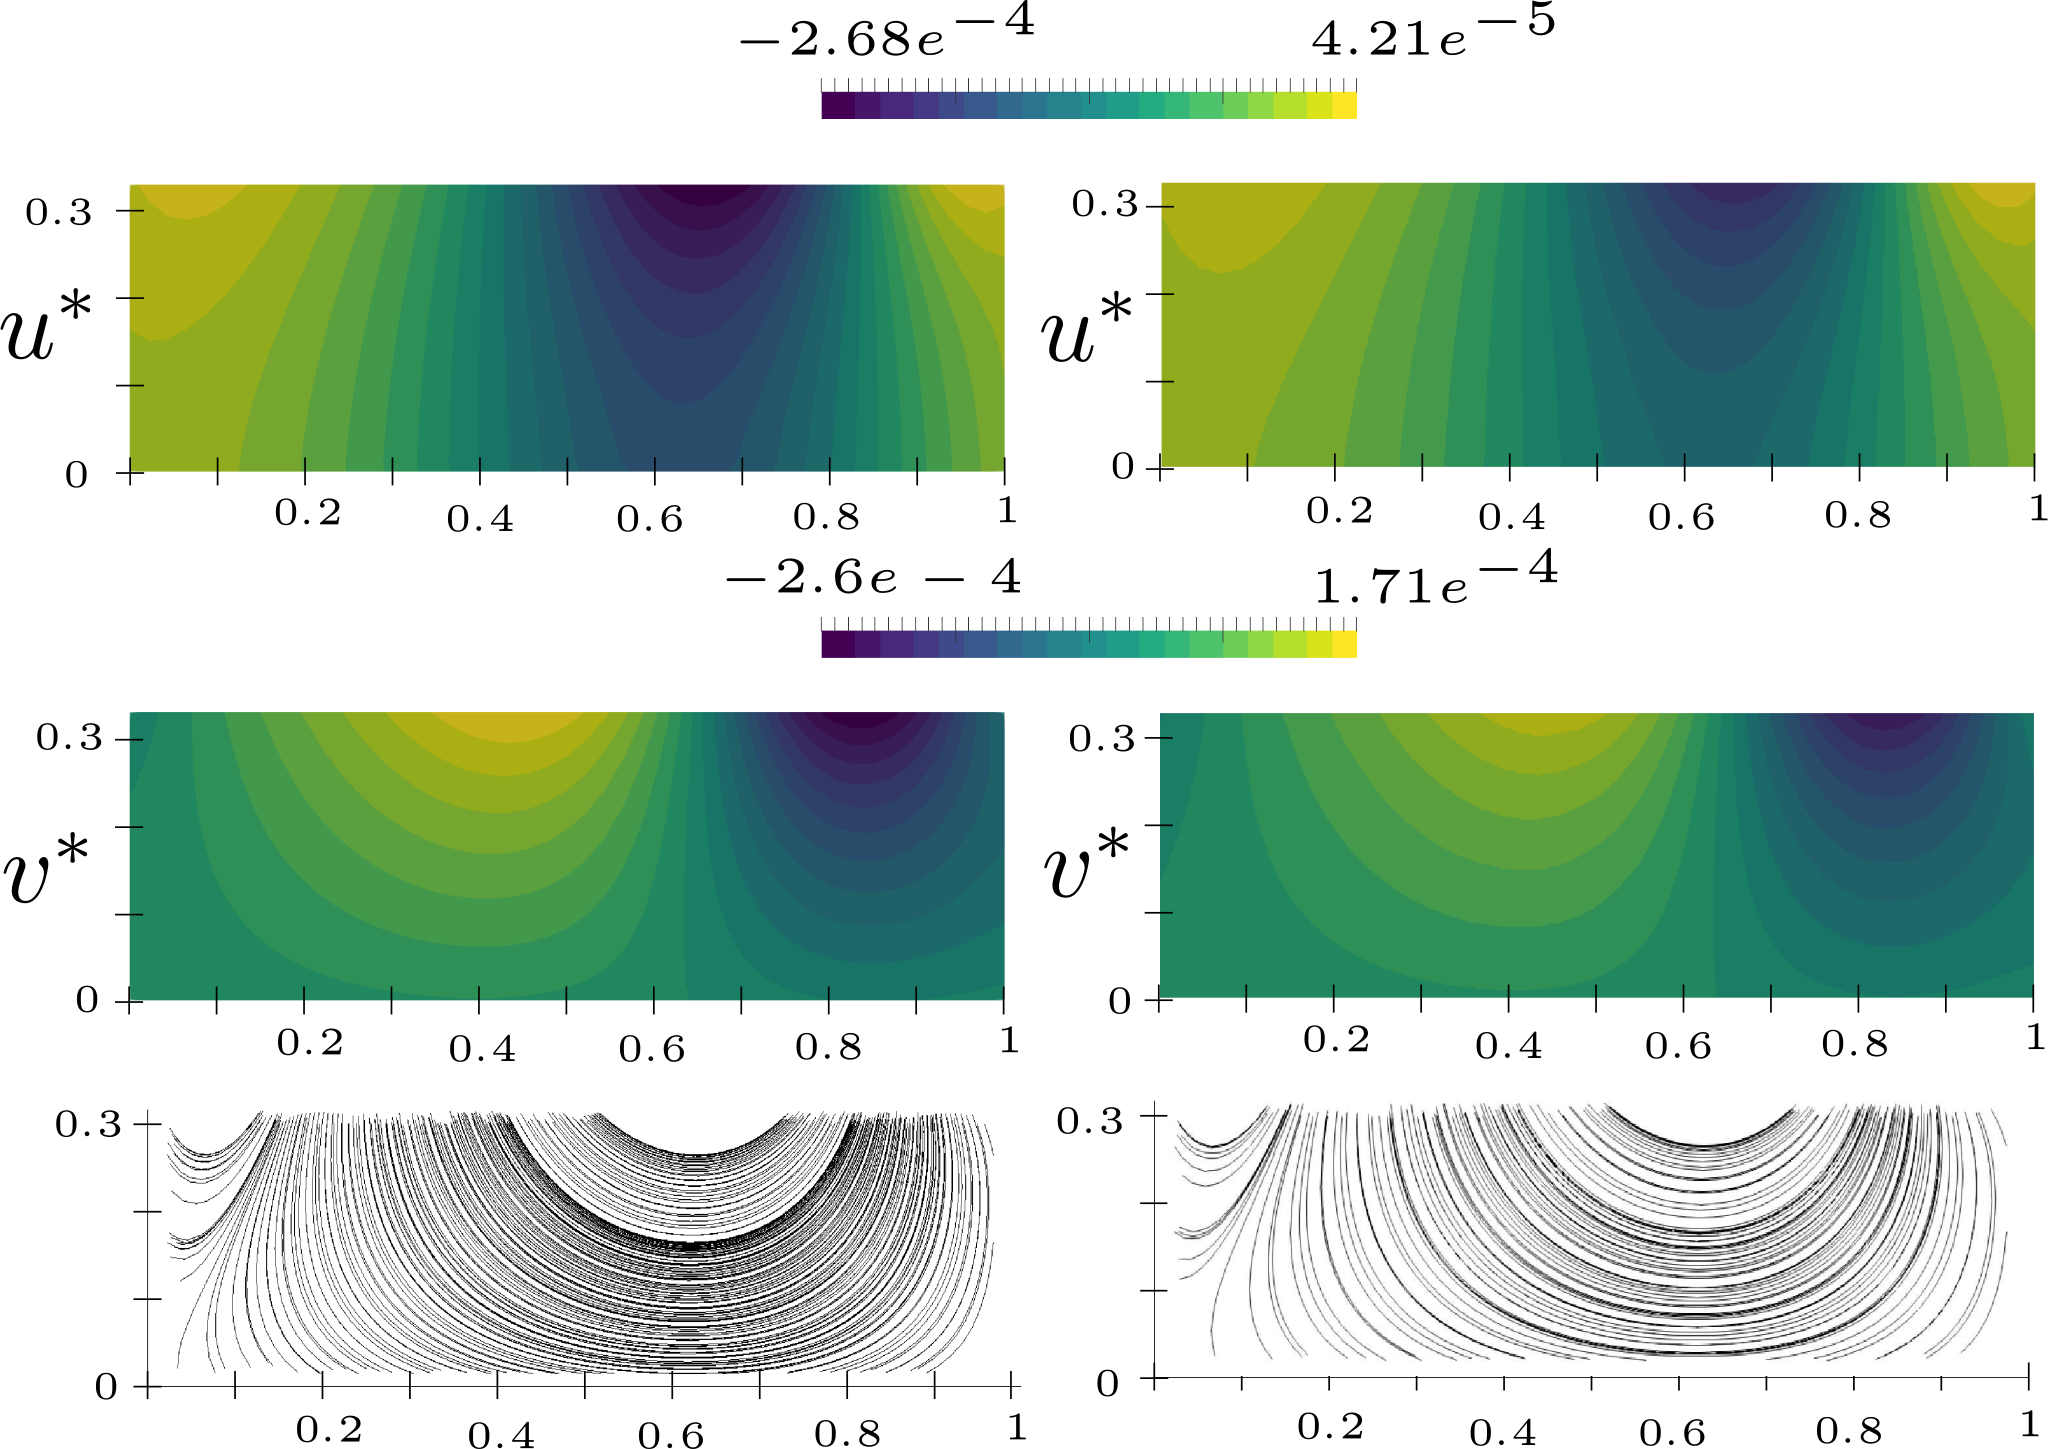
\includegraphics[width=1\linewidth]{chapter_5/figure/re100/vans_u}
	\caption{Left: VANS approach. Right: Homogenized DNS approach. The figures show, from top to bottom, the horizontal velocity the vertical velocity and the streamlines inside the porous domain $\Omega_p$}
	\label{fig:100_u}
\end{figure}

The DNS approach is used as reference case for the comparison. At Reynolds number equal to $100$ we have a good agreement in the velocities and pressure gradients fields. The contours and the location of the local minima and maxima are the same for the two approaches. If we look at the numerical values, for some fields the relative errors are not negligible; however, they are in mean always below $10\%$. Also the flow path inside the porous domain is in good agreement with the DNS data.
Some differences between the two models have to expected since in the VANS approach the micro-scale flow behavior is modeled. This means that some of the details that the full DNS is able to retain, are lost in the macroscopic approach. 

\begin{figure}[H]
	\centering
	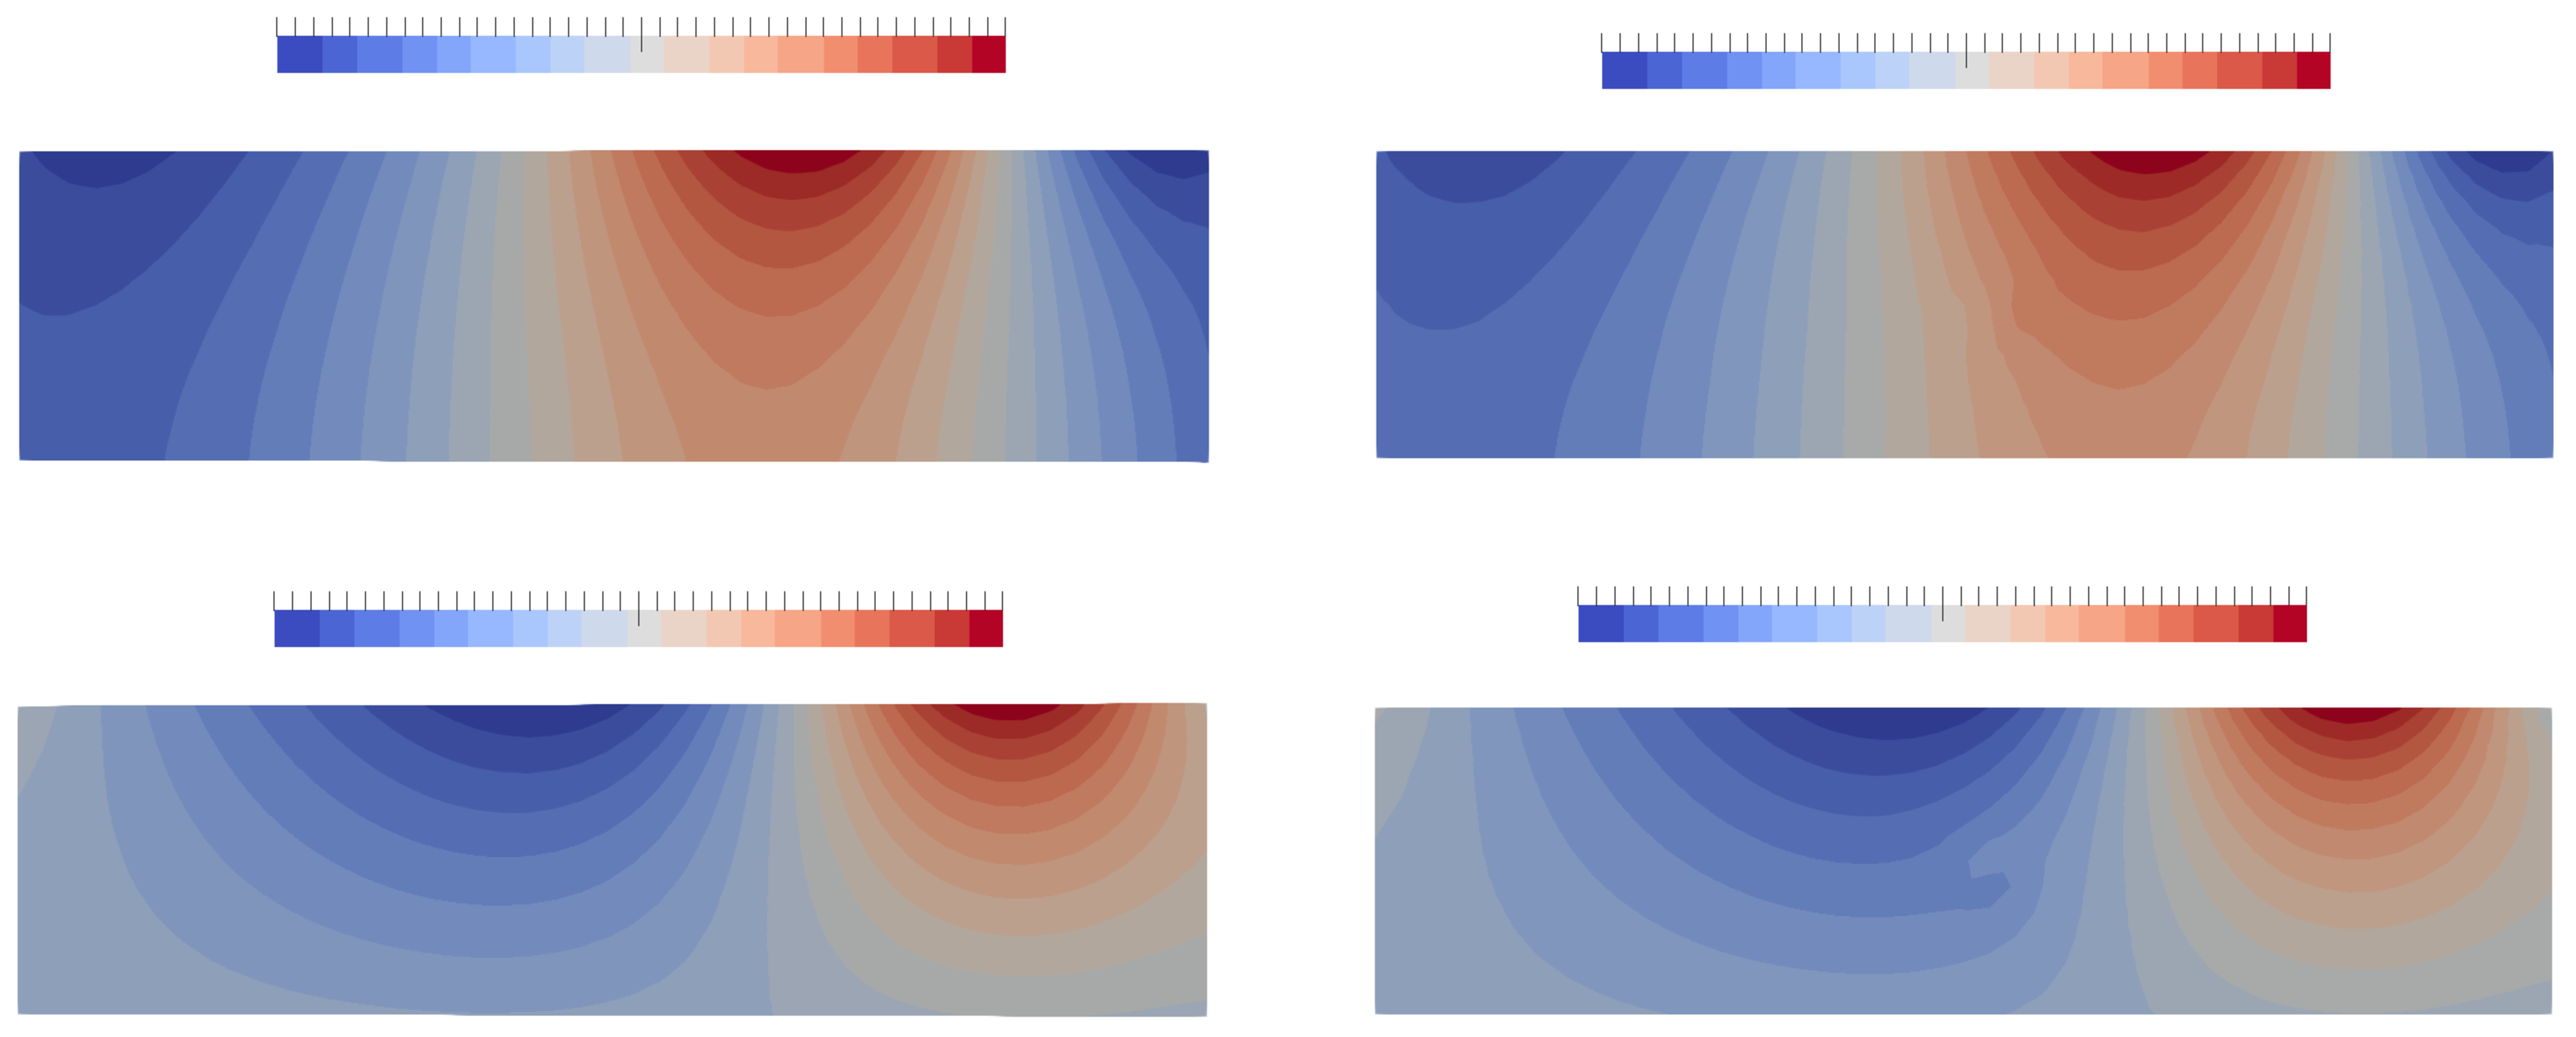
\includegraphics[width=1\linewidth]{chapter_5/figure/re100/vans_p}
	\caption{Left: VANS approach. Right: Homogenized DNS approach. The figures show, from top to bottom, the horizontal and the vertical component of the pressure gradient inside the porous domain $\Omega_p$}
	\label{fig:100_p}
\end{figure}


\subsection{Cavity $Re=1000$ comparison}

The same case and comparison has been done also for a Reynolds number equal to $Re=1000$.
For this case the same conclusion as the previous case are confirmed. Some of the relative errors are even smaller compared to the previous Reynolds number case. This support the robustness of our model in this range of Reynolds numbers.
These two solutions of the cavity problem shown that varying the permeability and the porosity in a linear manner through the interface is an acceptable choice when using the penalization method.

\begin{figure}[H]
	\centering
	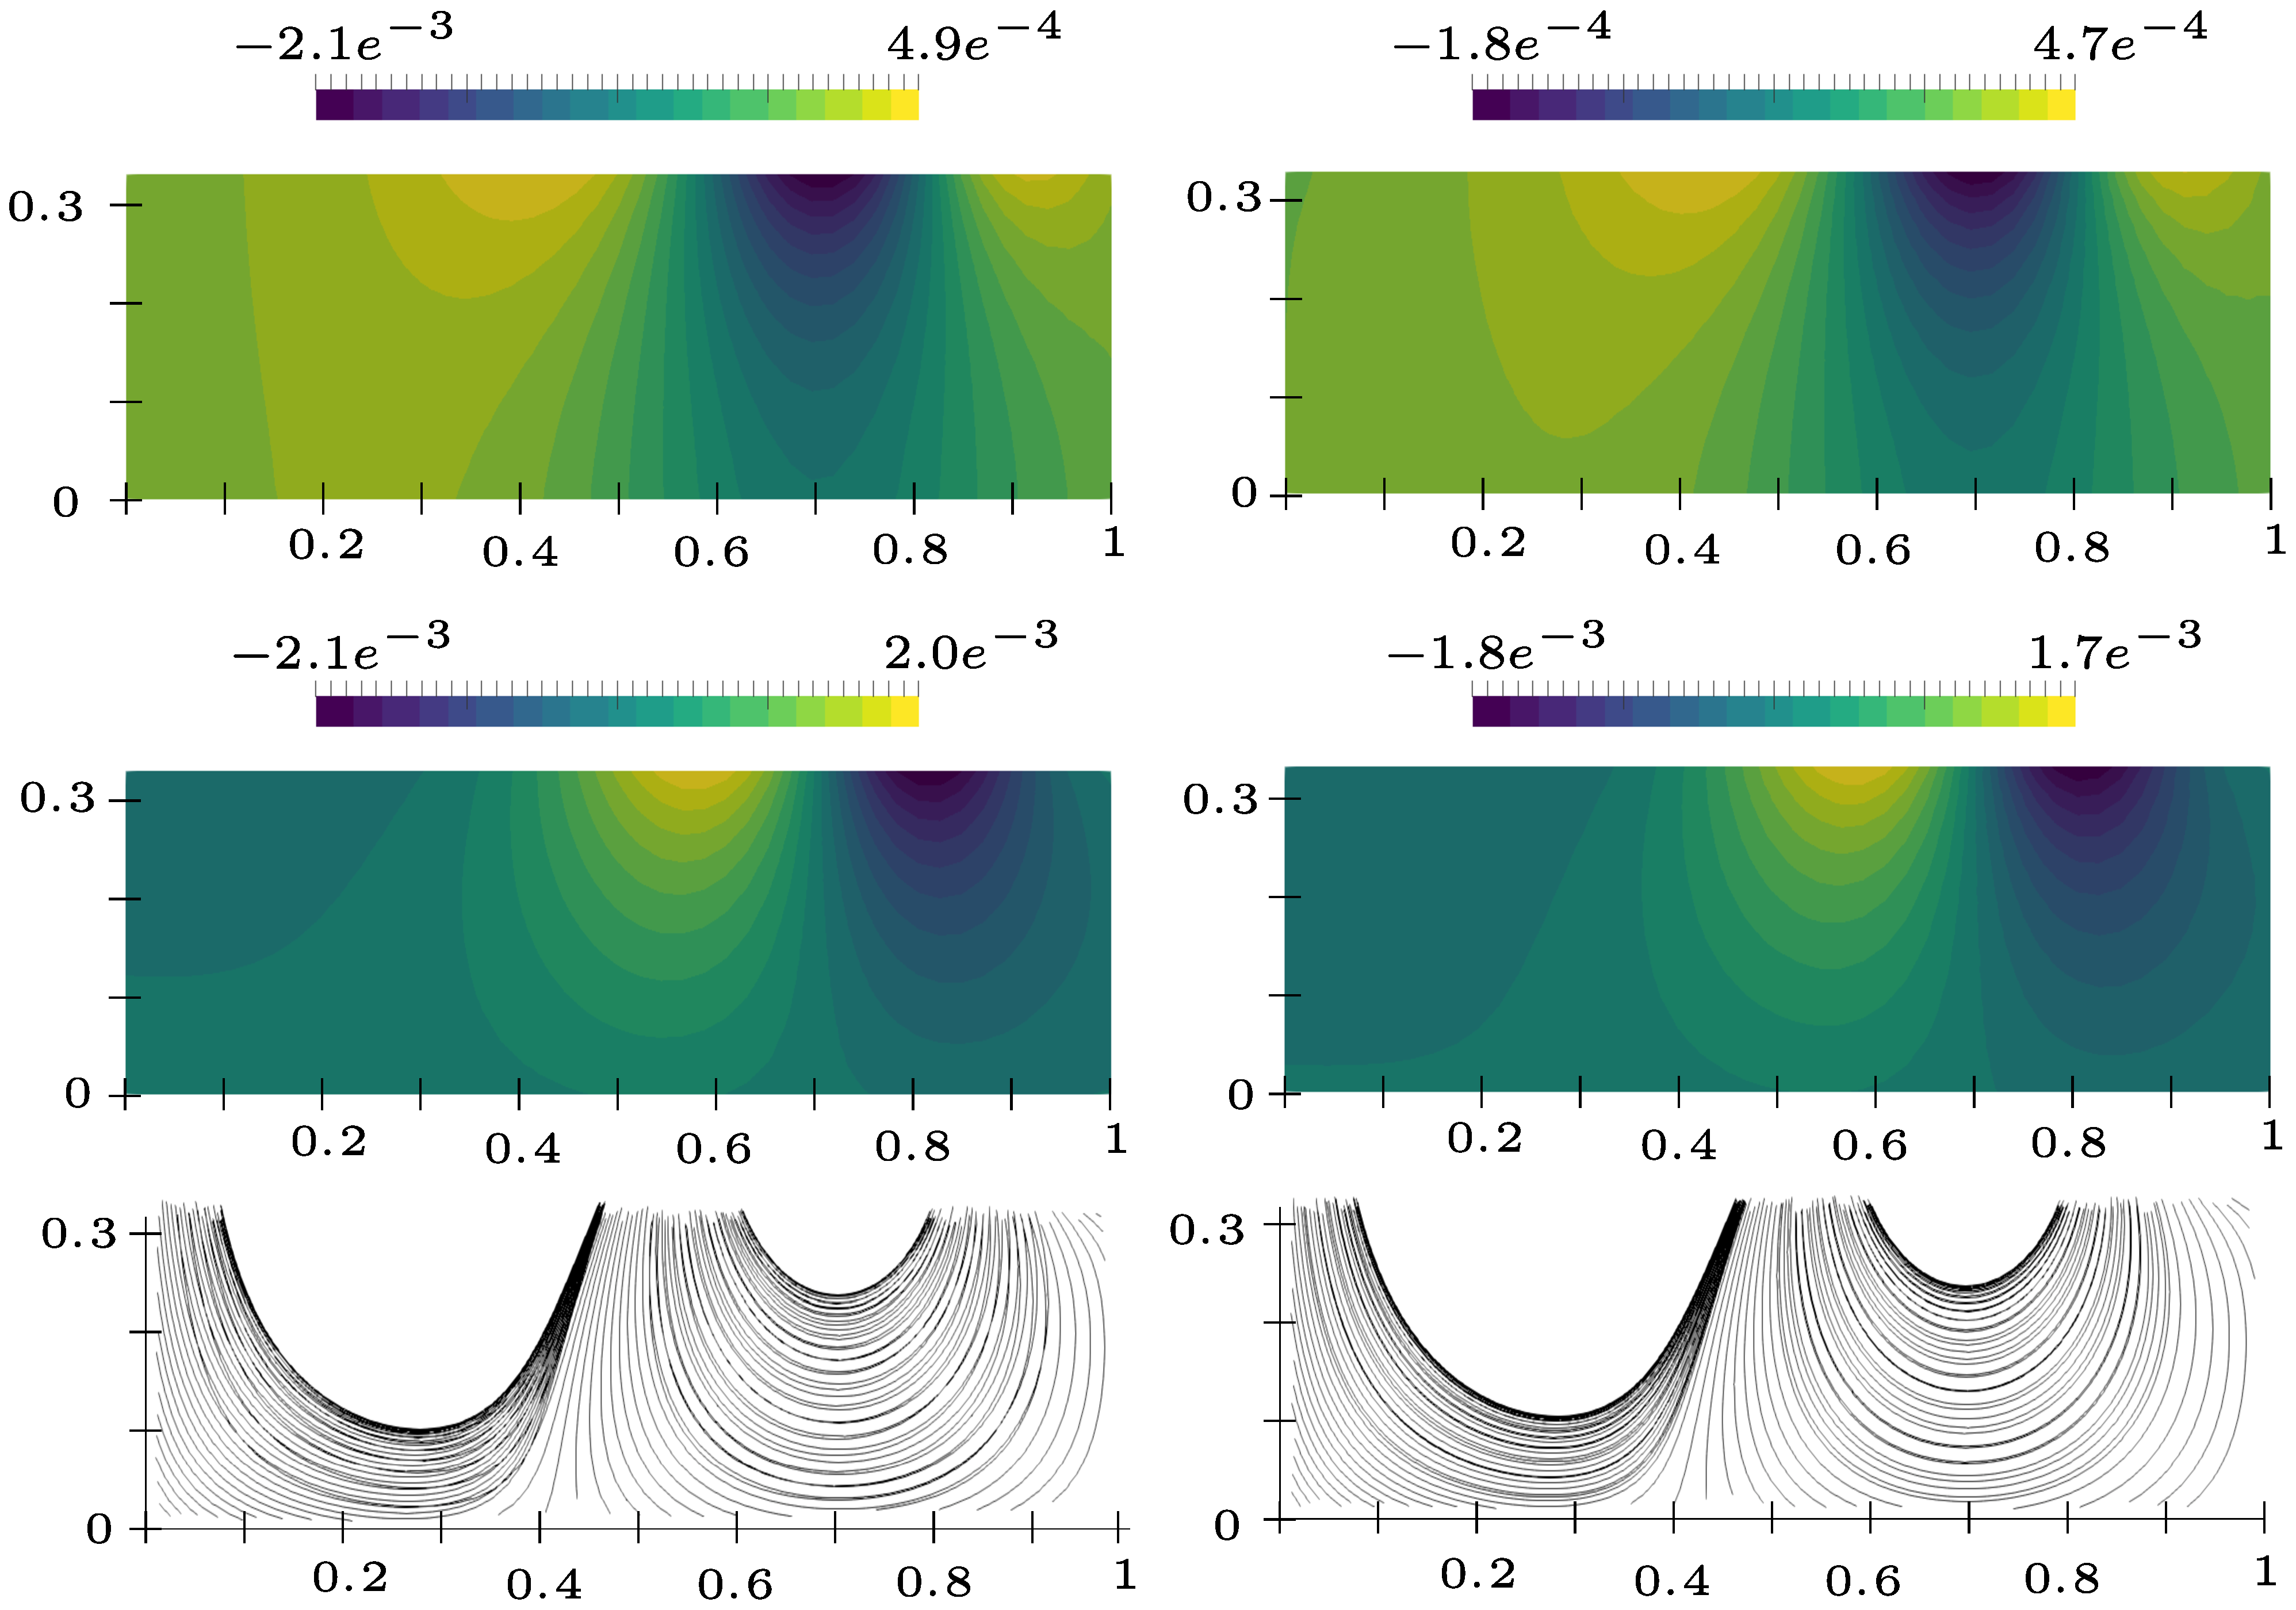
\includegraphics[width=1\linewidth]{chapter_5/figure/re1000/vans_u}
	\caption{Left: VANS approach. Right: Homogenized DNS approach. The figures show, from top to bottom, the horizontal velocity the vertical velocity and the streamlines inside the porous domain $\Omega_p$}
	\label{fig:1000_u}
\end{figure}

\begin{figure}[H]
	\centering
	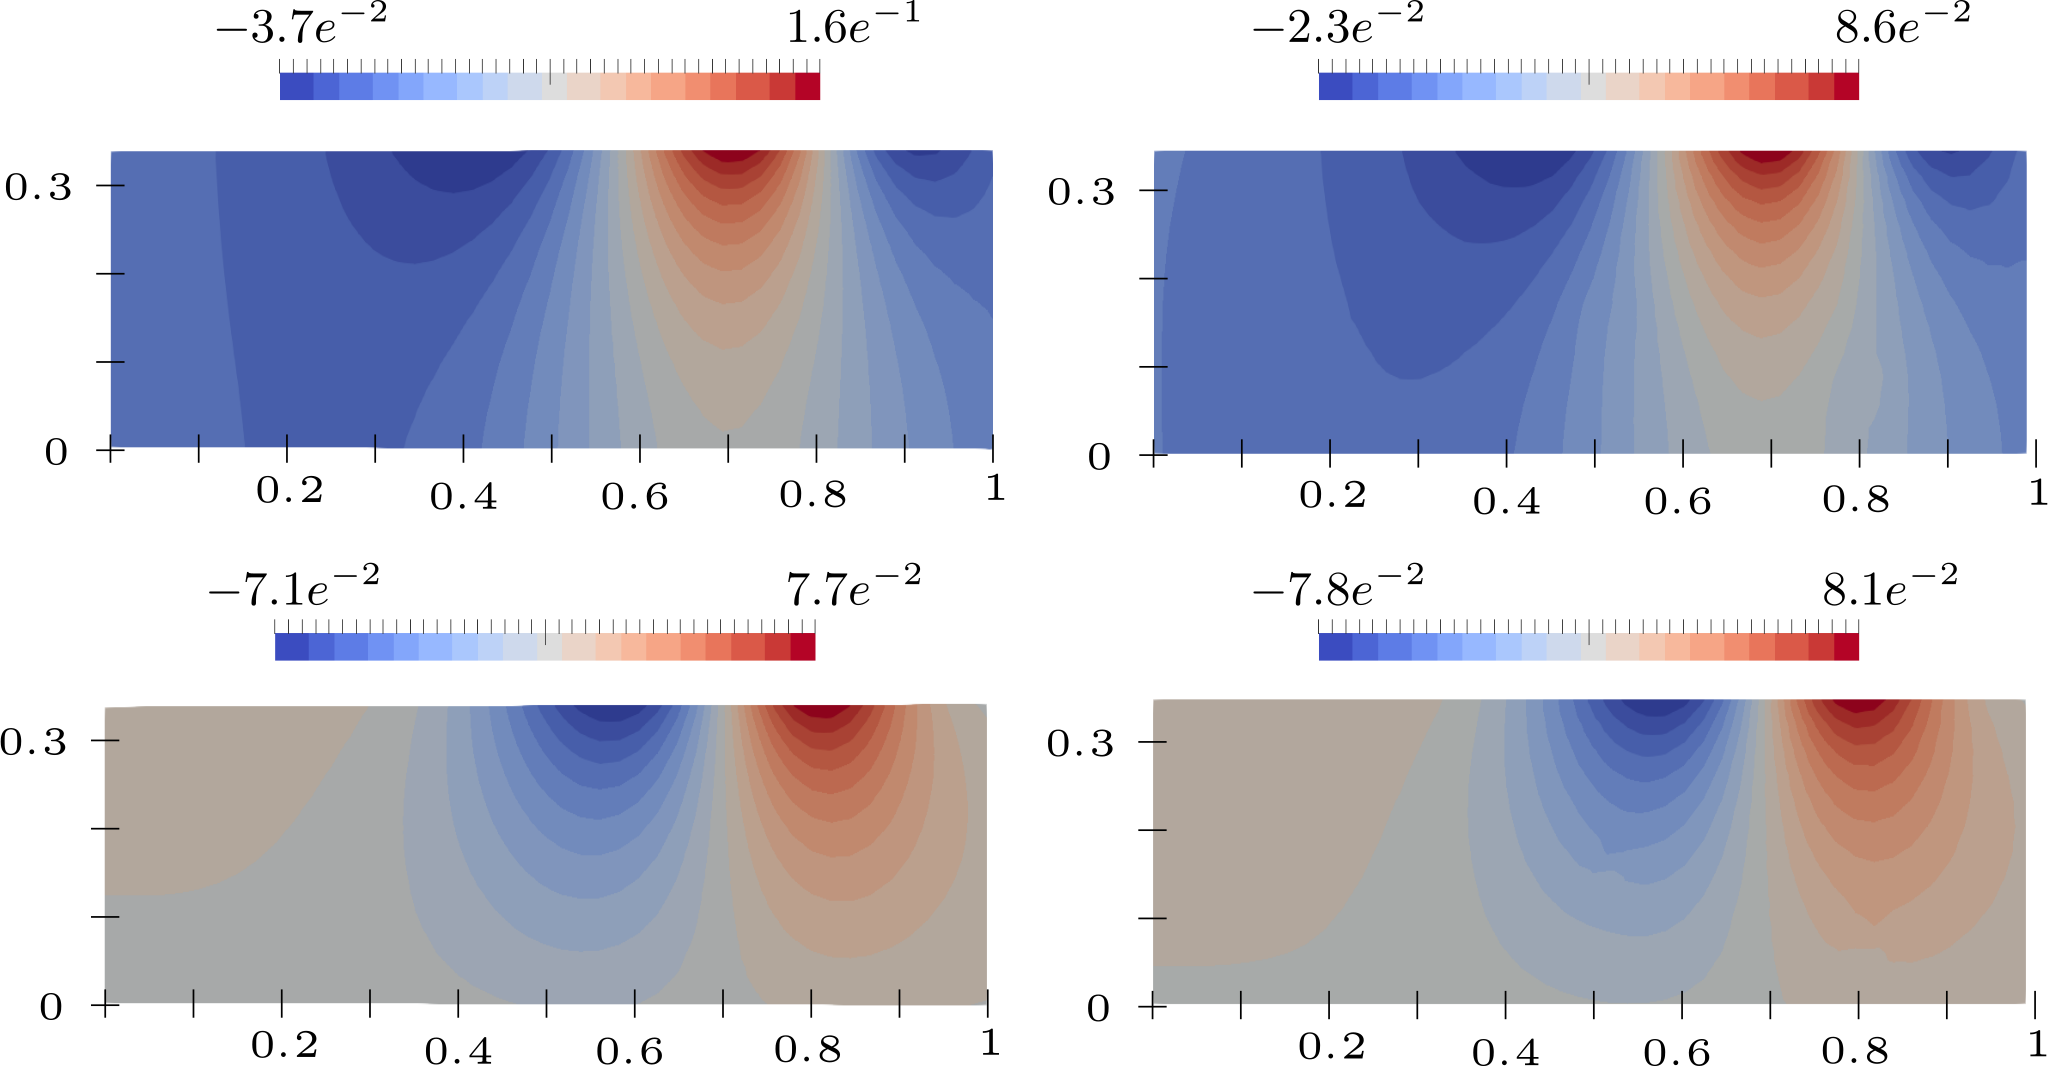
\includegraphics[width=1\linewidth]{chapter_5/figure/re1000/vans_p}
	\caption{Left: VANS approach. Right: Homogenized DNS approach. The figures show, from top to bottom, the horizontal and the vertical component of the pressure gradient inside the porous domain $\Omega_p$}
	\label{fig:1000_p}
\end{figure}

\begin{figure}
	\centering
	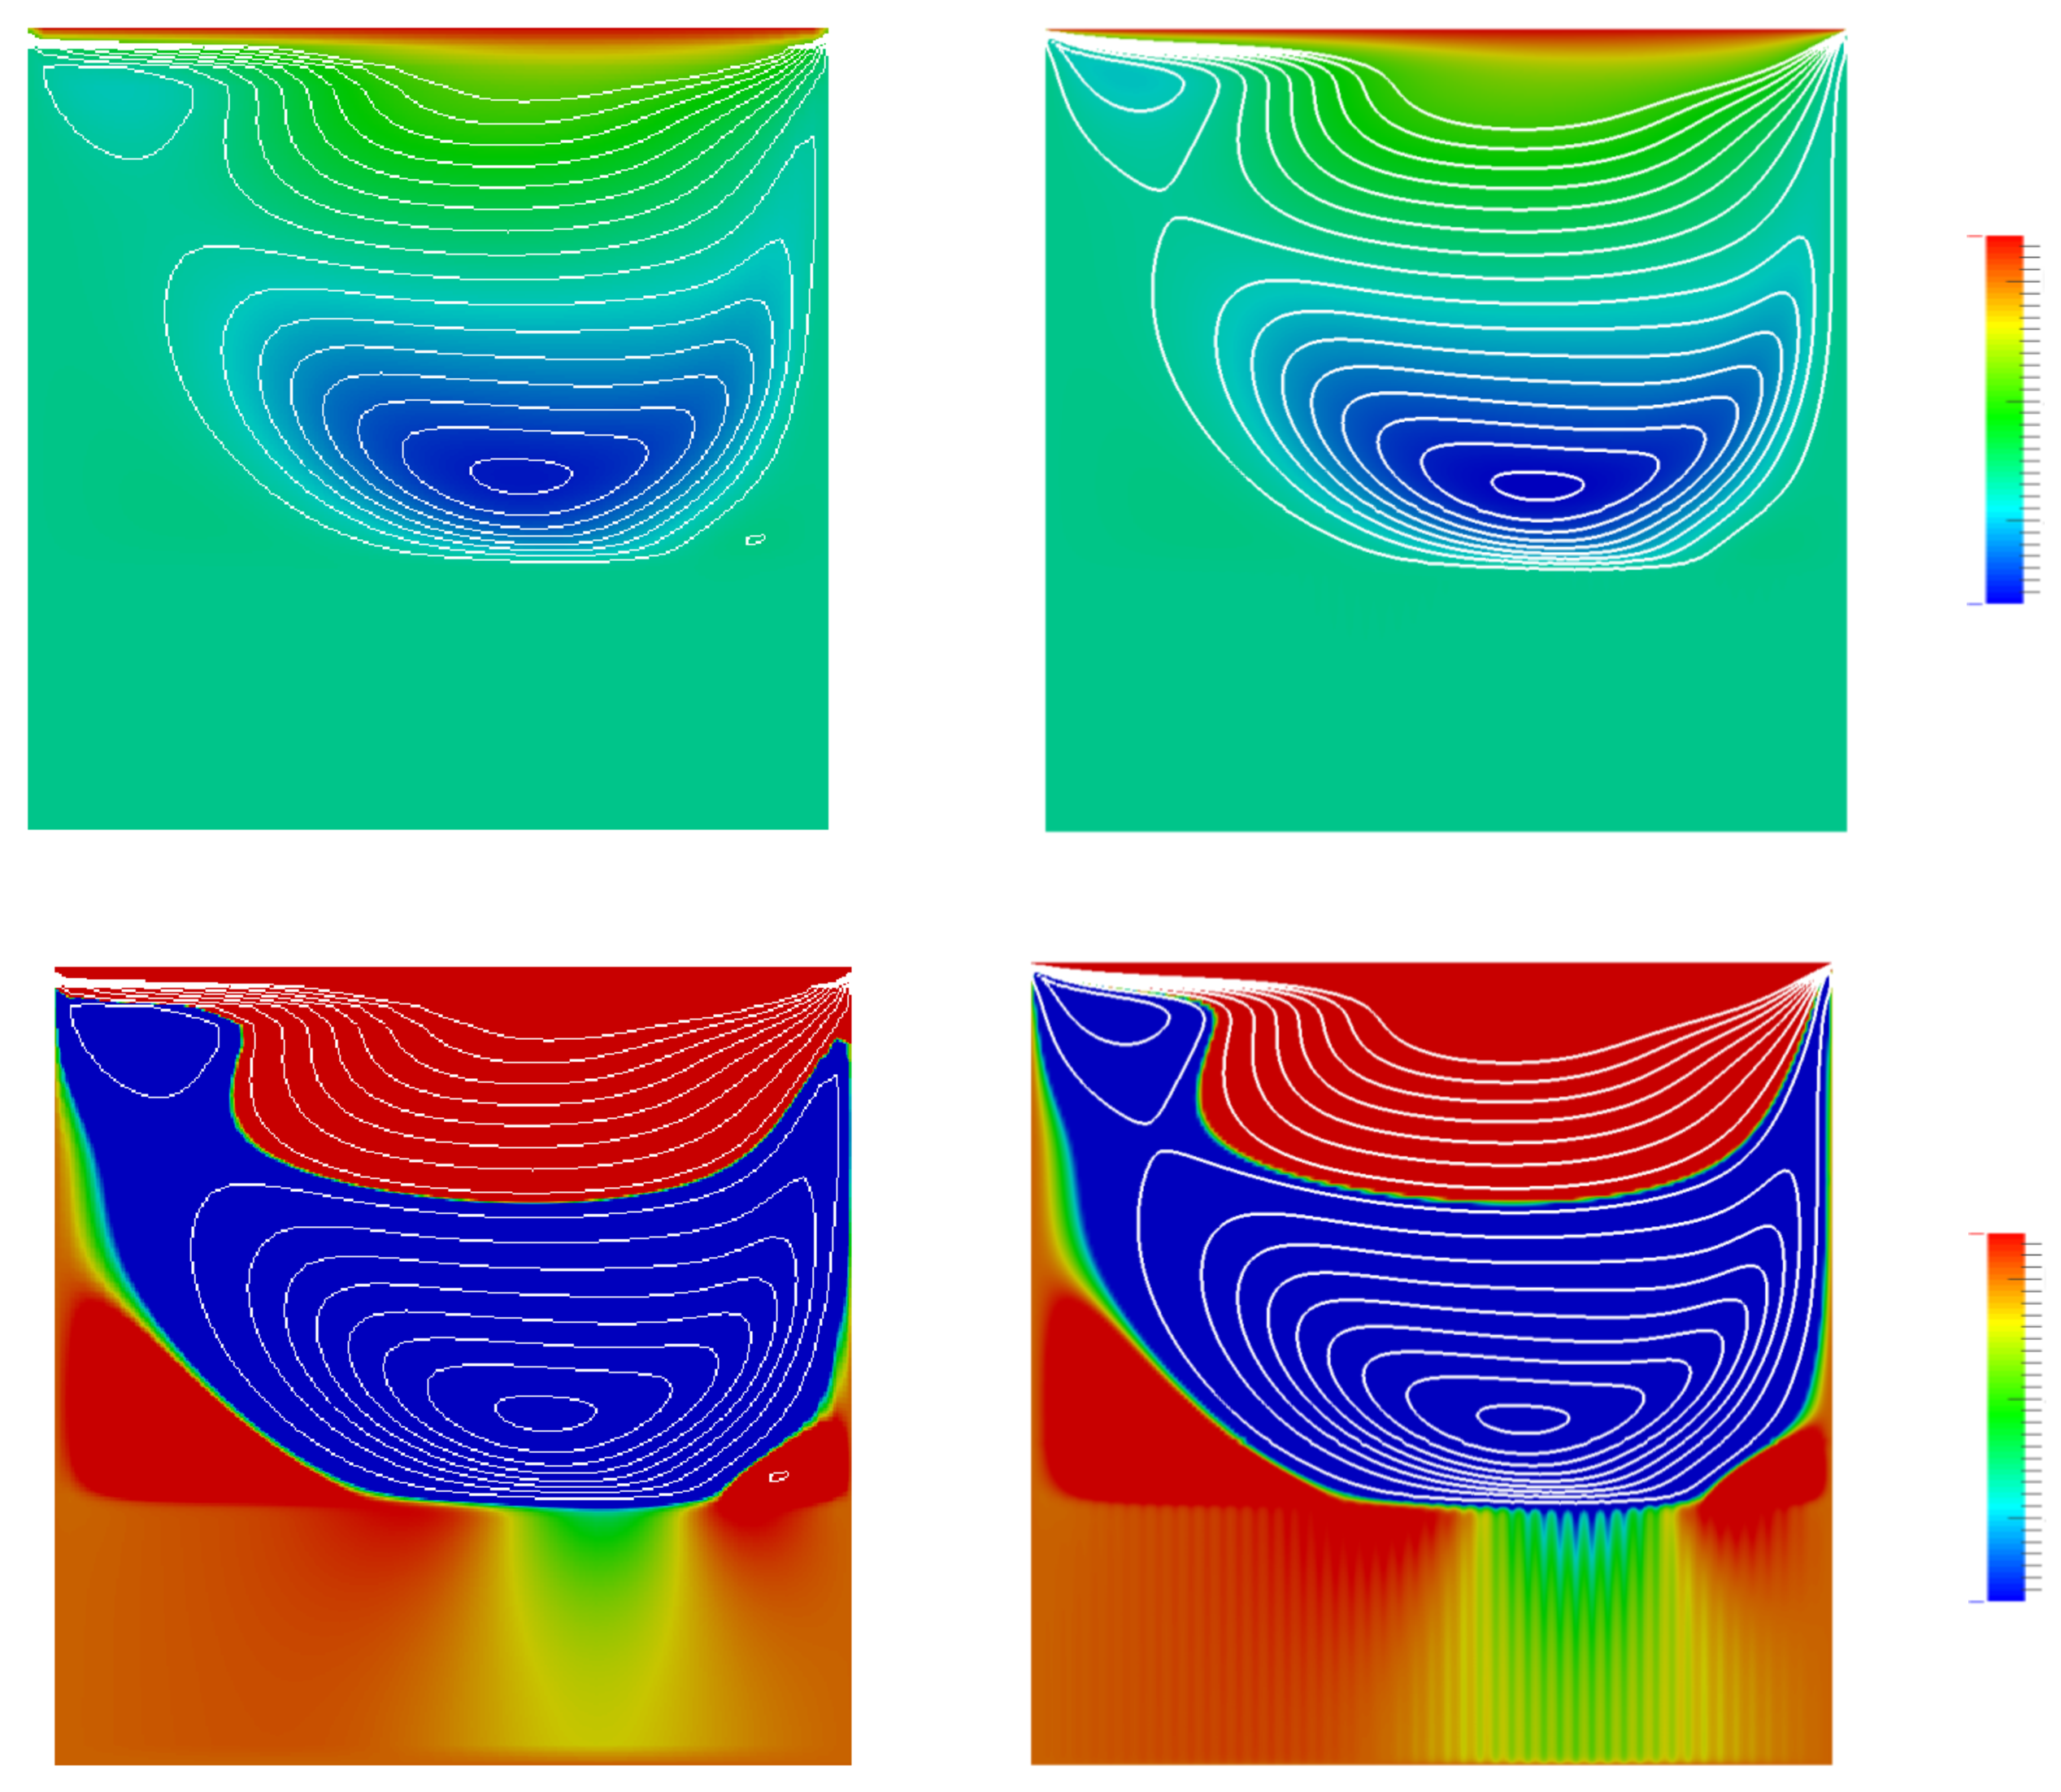
\includegraphics[width=0.9\linewidth]{chapter_5/figure/re_100_big/ux}
	\caption{big comparison horizzontal vel}
	\label{fig:ux}
\end{figure}

\begin{figure}
	\centering
	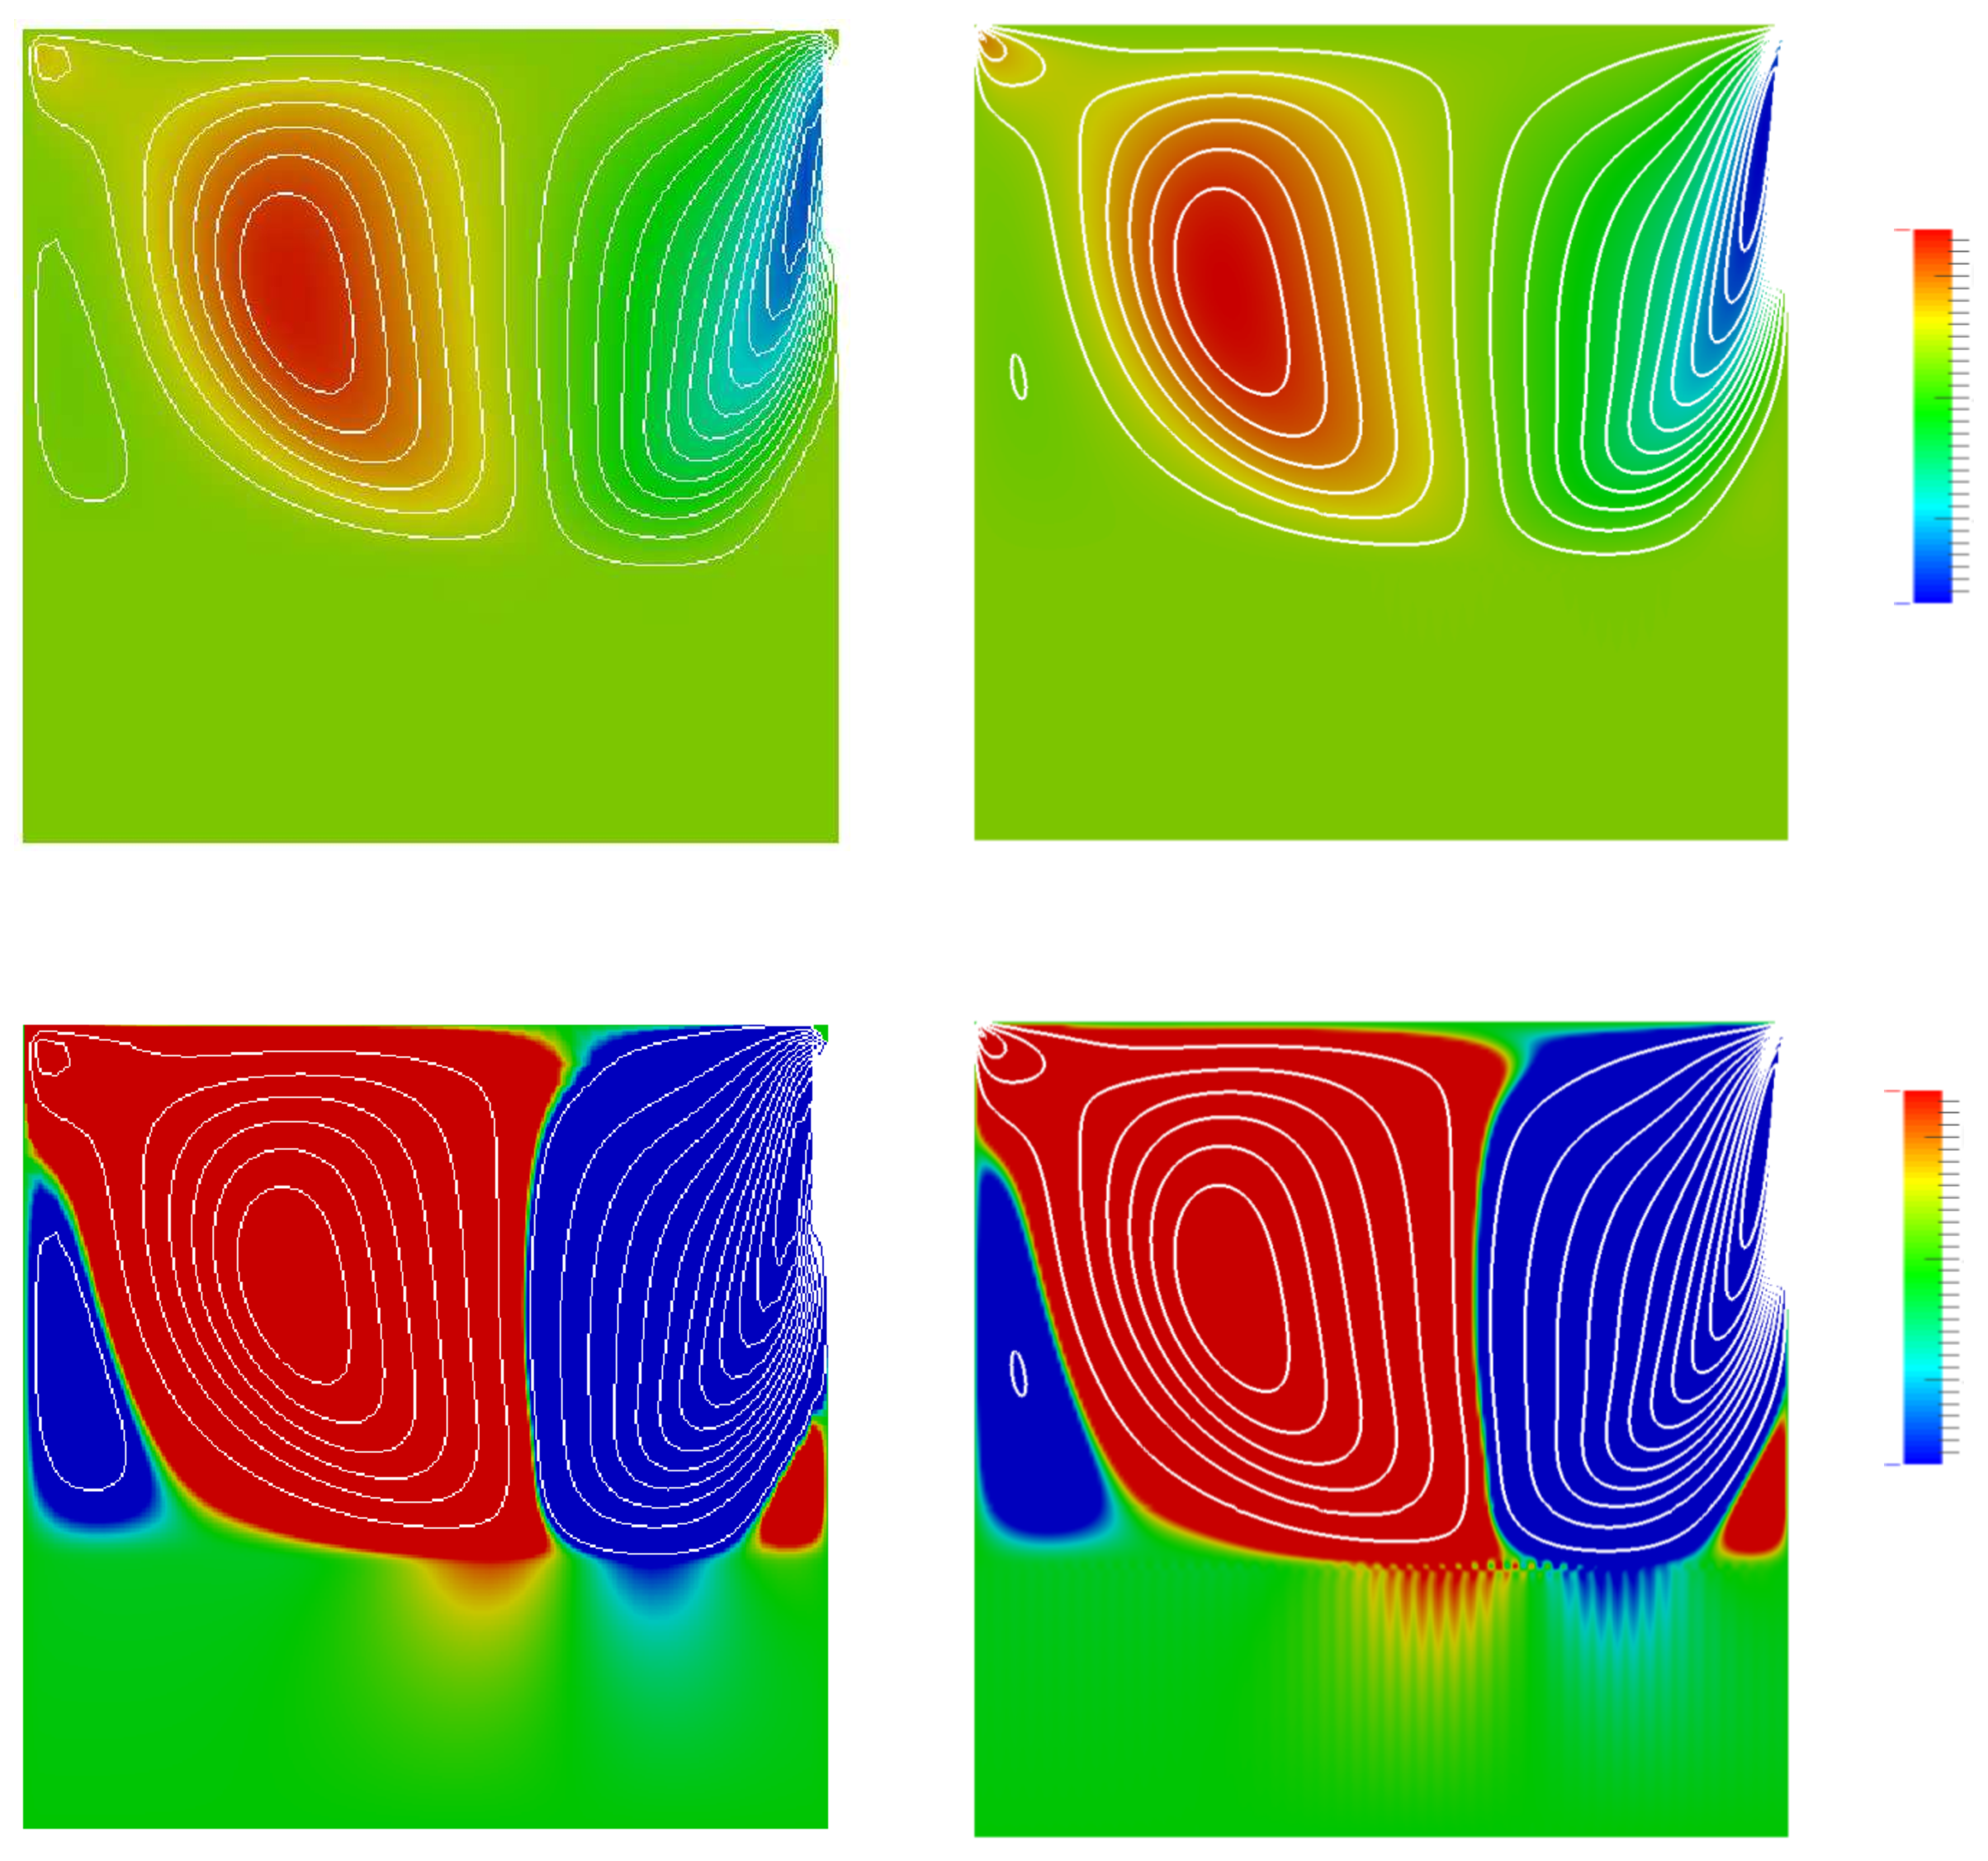
\includegraphics[width=0.9\linewidth]{chapter_5/figure/re_100_big/uy}
	\caption{big comparison vertical vel}
	\label{fig:uy}
\end{figure}


\subsection{Cavity $Re=5000$ using $\mathbf{H}$ metamodel}
\label{pr:mata_cav}
In our previous simulations the metamodel for the effective permeability has not been applied.  The metamodel in chapter \ref{ch:4} was built for a porous medium made of staggered cylinders. So it would not be applicable when the porous medium is made by regular arranged cylinders.

In order to test how the effective permeability variation would impact our model we show the solution for another test case. In the same cavity geometry as before the system \eqref{eq:vans_cav} is solved with or without the kriging metamodel for the effective permeability.

We have observed that at low pore Reynolds number the effective permeability is practically not sensitive to variations of flow direction and/or magnitude\footnote{see figures \ref{fig:08_H}, \ref{fig:08_H} and \ref{fig:08_H} in chapter \ref{ch:4}.}.
For this reason also the Reynolds number has been increased to $5000$, that is still in the stationary regime but near the transition limit (\citet{peng2003transition}).

\begin{figure}[h]
	\centering
	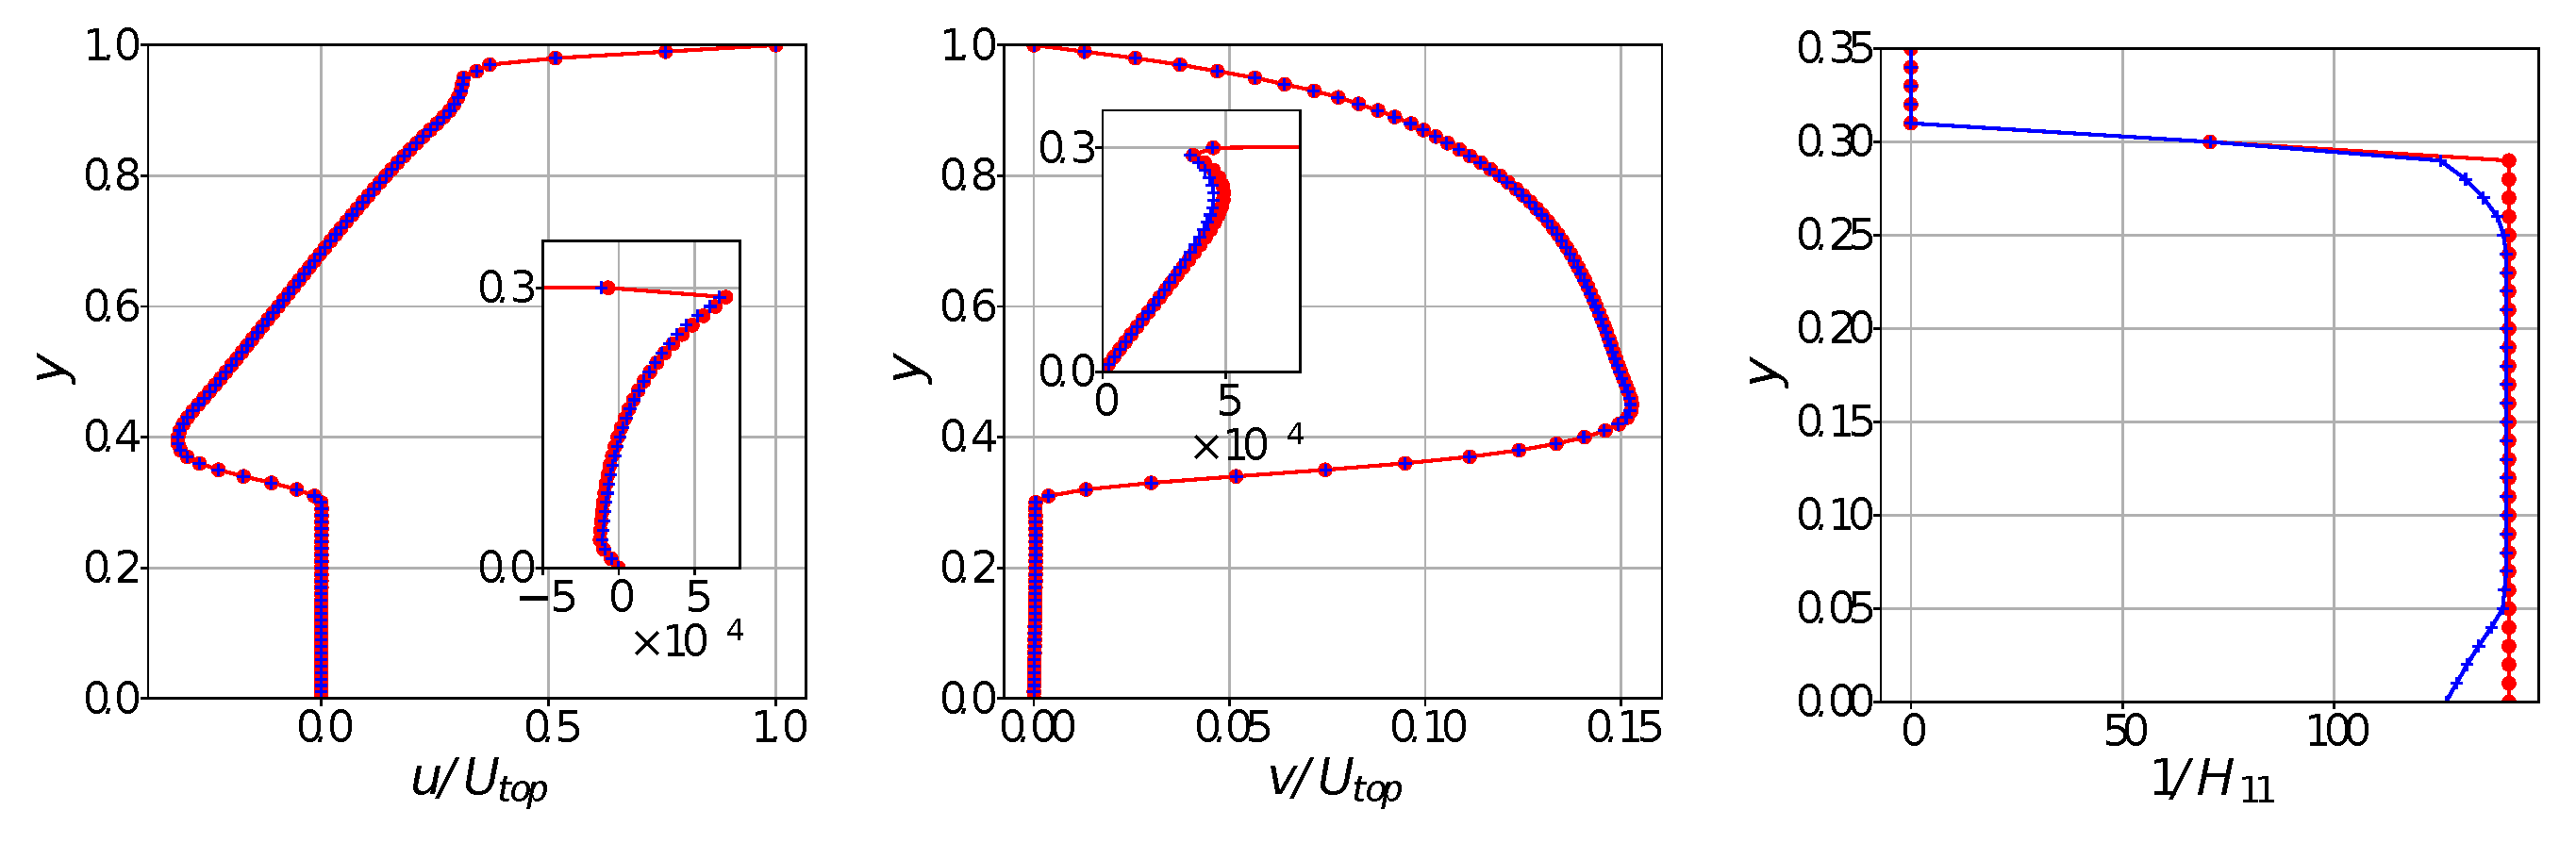
\includegraphics[width=0.9\linewidth]{chapter_5/figure/cav_5000}
	\caption{Left: horizontal velocity component. Center: vertical velocity component. Right: Effective permeability $11$ component. The three fields have been sampled at the center of the cavity, $x_1=0.5 \,L$. The blue line represents the solution for the system \eqref{eq:vans_cav} with the kriging metamodel for the effective permeability, the red line is the solution of the same system with the model switched off.}
	\label{fig:cav5000}
\end{figure}

Figure \ref{fig:cav5000} shows the velocity and permeability profiles for a sample cut made at the center of the cavity at $x=0.5\,L$.
It is clear that the macroscopic velocity is not affected by the different treatment of the permeability, as a matter of fact the two velocities can be superposed almost precisely.
However, the inverse of the effective permeability component show some differences. At the interface it is possible to see also how the trend of the two different treatments look like at the interface. The permeability starts to increase at a deeper vertical position than the case without metamodel. This is caused by the vertical angle $\phi$ that is near $90^\circ$ at that point because of the fluid penetration. The analysis made in chapter 4 shows that the permeability increases when the angle $\phi$ increases.
However the value of the permeability deep in the medium is almost the same. 
In any case even if there are some differences in the permeability profiles this seems not to affect the average velocities.

The fact that with the kriging metamodel the same linear profile as equation \ref{eq:permeability_fun} is retrieved is another confirmation that the linear variation is acceptable.

%\footnote{The dots in the figure \ref{fig:cav5000} lines are used only to ease the read of the plots and do not correspond at the mesh nodes (that are too much to be represented clearly).}

\section{Separated flow between hills}
In chapter 1 we have presented some flow examples where a porous media layer in the leeward side of a bluff body can reduce the separation extension. In order to test the effectiveness of our model to make predictions in this sense, the flow over periodically arranged hills has been chosen as test problem. This configuration has already been investigated experimentally and numerically and is a classical CFD problem, now standardized by the ERCOFTAC committee.
It is used as a benchmark case to investigate the ability of DNS, RANS and LES models to resolve separation from a curved geometry.
The flow field features a large separation bubble caused by the curved surface of the hill and a natural reattachment in the flat part between the two hills crests. 
The flow is assumed to be periodic and two dimensional, at the Reynolds number tested. Numerous DNS and LES works can be found in literature with Reynolds numbers up to 10000 (\citet{chang2014simulations}, \citet{breuer2005issues} \cite{breuer2009flow}, \citet{almeida1993wake} and \citet{temmerman2001large}).
This test case has been studied with two main objectives: to test the modeling and simulation issue related to our VANS solver and the physical capacity to reproduce the flow field behavior. 
Our idea is to extend the hill profile with a porous media layer and assess how the separation bubble is modified by the layer presence.
We have tested a small Reynolds number case in the laminar regime. The problem has been chosen especially for the possibility to future extend the study towards higher Reynolds numbers since a lot of data can be found in the literature to validate the results.

\subsubsection{Geometry and conditions}
The geometry of the problem is depicted in figure \ref{fig:mesh_hill}. It is two dimensional since the Reynolds number considered is in the laminar regime and the flow does not present any three dimensional characteristics in this range. The dimension of the hill crest and extensions are also showed in the same pictures being rendered adimensional with the hill crest height. The chosen dimensions of our setup are: $L_x = 9.0$, $L_y = 3.036$ and $h = 1$ where $x,y,z$ are the streamwise, wall-normal and spanwise direction, respectively. We solve the flow inside of a single streamwise periodic segment and thus cover solely one complete hill region from crest to crest.
Between one hill and the next one there is a flat plate region of extension $5h$. The pressure-induced separation takes place from the first hill curved surface and reattachment is observed at the flat plate part between the two hills.

The hills profile is described by a polynomial parametric curve function of the streamwise direction $y_{hill} = f(x)$. The specific coefficients and definition can be found in \citet{almeida1993wake}. This geometry is also named \textbf{base} case in the following text.

The problem is discretized using the finite volume method implemented in OpenFoam and the mesh used is shown in figure \ref{fig:mesh_hill}. The mesh is purely made of hexahedral cells and counts 25000 elements in the two dimensional version. It is possible to download it at \url{https://turbmodels.larc.nasa.gov/Other_LES_Data/2dhill_periodic.html}. The resolution has been already validated in DNS and LES computations so it has not been further investigated here.

\begin{figure}[h]
	\centering
	\includegraphics[width=1\linewidth]{chapter_5/figure/mesh}
	\caption{Domain of the problem and mesh used to discretize it. On the right side there is an enlargement of the zone on the hill curvature.}
	\label{fig:mesh_hill}
\end{figure}

The inlet and the outlet patches are connected with a periodic boundary condition; at the hill and flat plate surface the no-slip condition is imposed and finally at the top of the domain a slip condition is used.
The numerical setup for the numerical scheme and linear solvers is the same as the DNS simulations in chapter 4, paragraph \ref{ph:numeric_setup}.

The equations solved are a slightly modified version of the VANS system \eqref{eq:vans_cav} in which the constant macroscopic pressure gradient is introduced as a source term in the momentum equation.

\begin{eqnarray}
\begin{cases}
\derp{\vbms}{t} + \dfrac{1}{\varepsilon} \nabla \cdot \left[  \vbmi  \vbmi \right] = -\dfrac{1}{\rho_{\beta}} \nabla \meani{\pb} + \nub \nabla^2 \vbmi \\ 
\qquad \qquad \qquad \qquad \qquad \qquad- \nub \varepsilon \mathbf{H}^{-1} \vbmi +\dfrac{\nub}{\varepsilon} \nabla \varepsilon \cdot \nabla \vbmi + \dfrac{\nub}{\varepsilon} \vbmi \nabla^2 \varepsilon - \mathbf{g}\\
\nabla \cdot \left(\varepsilon \vbmi \right) = 0\\
\vbms = 0 \qquad \textrm{at hill wall} \\
\derp{u}{y}=0 \qquad \textrm{at} \; y = 3.035\,h\\
\vbms|_{x_1 = 0} = \vbms|_{x_1 = 9h} \\
\pbms|_{x_1 = 0} = \pbms|_{x_1 = 9h} 
\end{cases}
\label{eq:sys_hill}
\end{eqnarray}

In the system \eqref{eq:sys_hill} the flow is driven by the source term $\mathbf{g}$ and the Reynolds number is computed a posteriori in the following manner:
$$
R_e = \dfrac{U_b h}{\nu},
$$
where $U_b$ is the velocity in the top left corner of the domain, just above the first hill.

The treatment for the porosity is the same as equation \eqref{eq:porsitity_fun} where in this case the $y_{itf}$ is described by two different profiles.
The first one, called \textbf{external}, is the same hill profile translated to the right by a length equal to $0.2\,h$ in the streamwise direction. This setup is used to test the case of a porous media layer on the external part of the hill. In this case the hill geometry is modified.

In the second case the interface profile $y_{itf}$ is exactly the hill profile at the same position and the solid part of the hill is translated in the direction $-x$ by $0.2\,h$. In this setup, denoted \textbf{internal}, the porous media layer has been inserted on the "inside" of the hill leeward side. It means that the total geometrical extension of the hill plus the porous media layer is the same as the base case described by $y_{hill}$.

The porous media layer has the same geometry of the one described in \ref{ch:4}, a series of cylinders in staggered arrangement. The cylinders are then arranged on the leeward side of the hill and they are aligned with the wall normal direction. Although their extension is not uniform, the line that goes through all the cylinders lid describe the curves $y_{itf}$ \textbf{external} and \textbf{internal}.

The two different porosity field arrangements are depicted in figure \ref{fig:por_gauss}. Where the porosity deep inside the medium, shown in green, is equal to $0.8$ and the exterior porosity field is equal to $1$ and is shown in purple.

\begin{figure}[h]
	\centering
	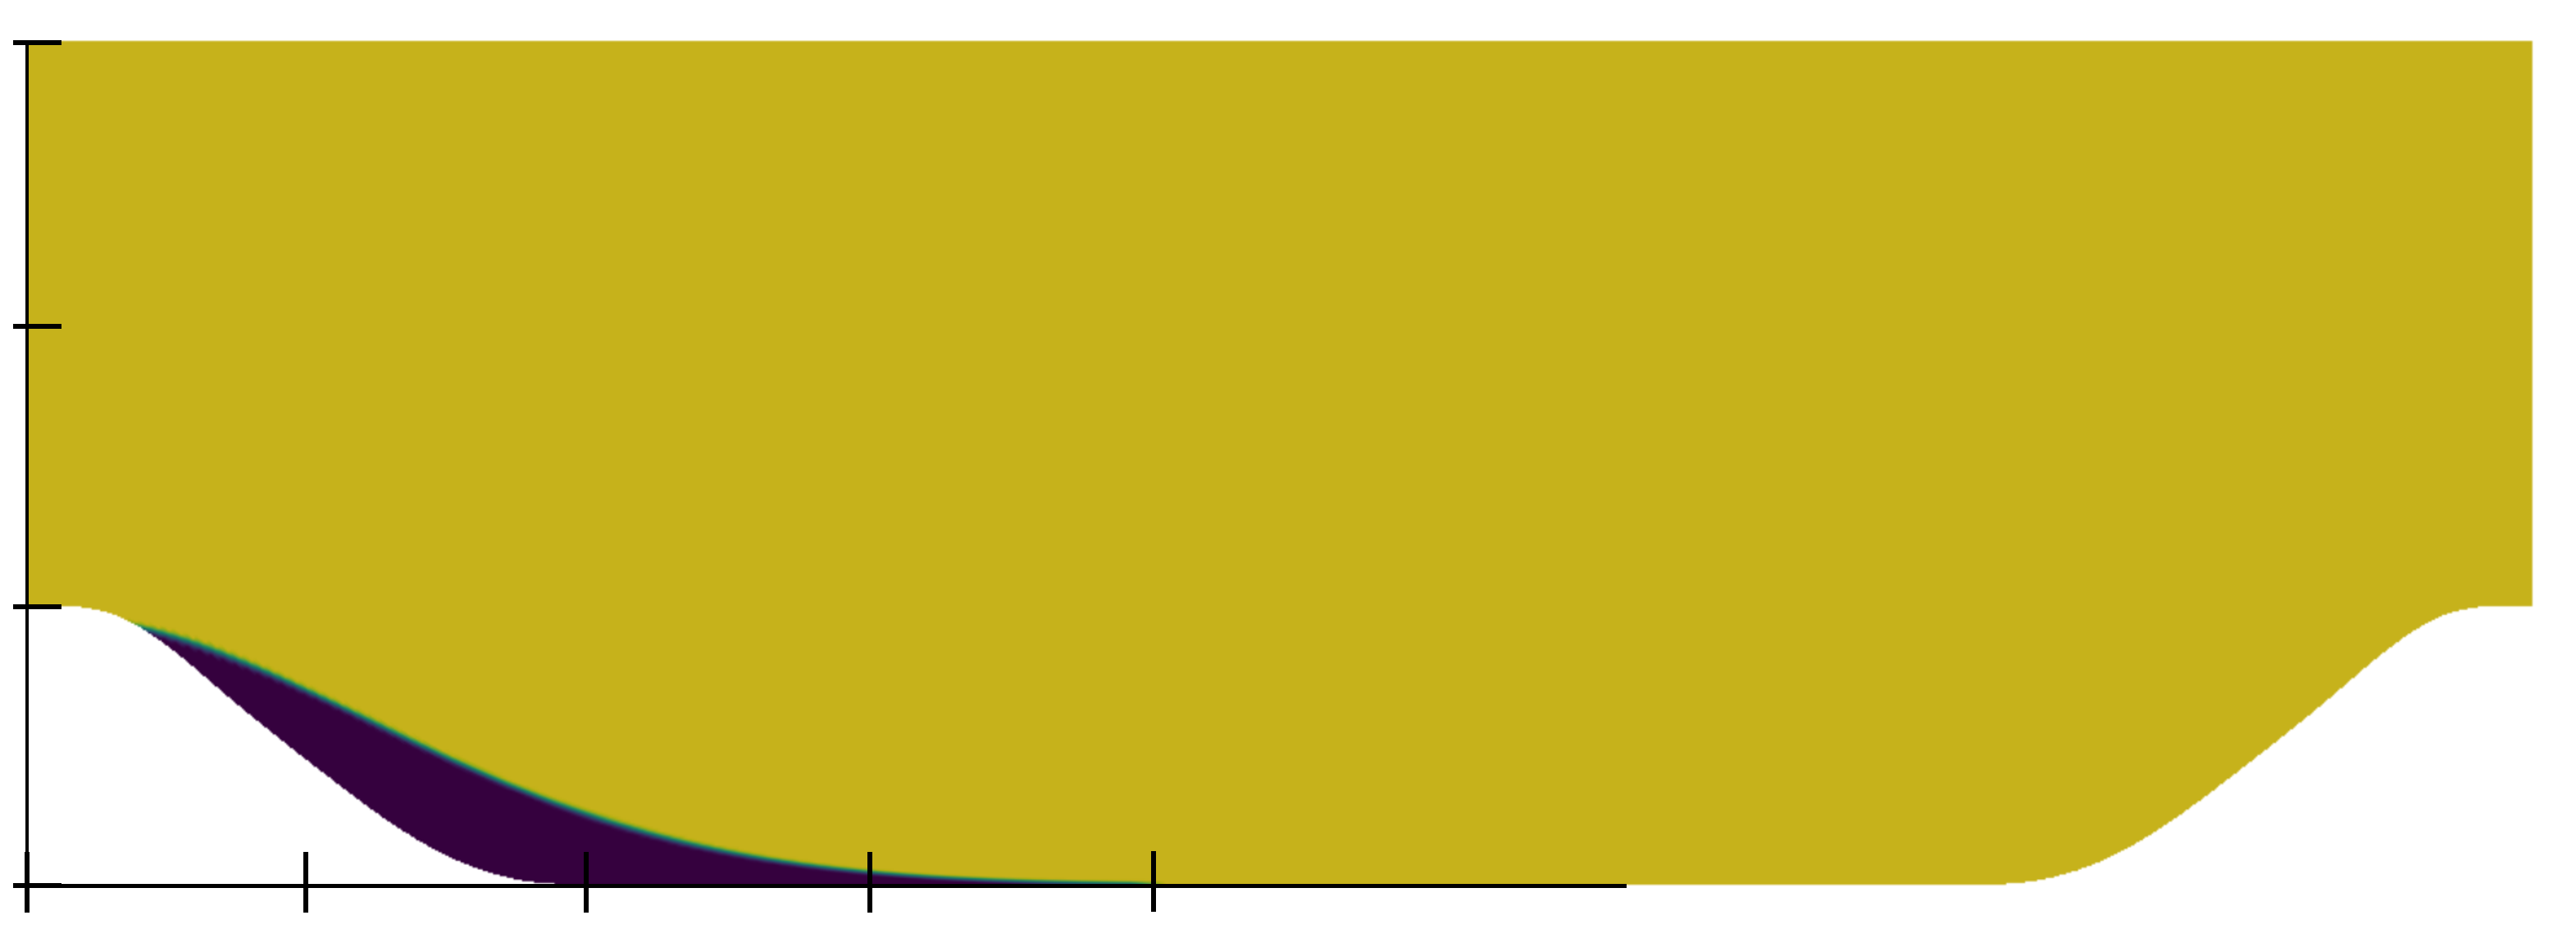
\includegraphics[width=1\linewidth]{chapter_5/figure/por}
	\caption{Porosity field in the leeward side of the first hill for the two different cases \textit{external} and \textit{internal}. The porosity in the deep medium is equal to $0.8$ and is colored in green, instead the porosity in the free fluid is equal to $1$ and it is colored in purple. On the left case, the \textit{external} one, the red line describes the hill profile of the base case and the white line describes the porous media interface. For the \textit{internal} case on the right the base hill profile and the porous media interface are the same one, and they are depicted in white.}
	\label{fig:por_gauss}
\end{figure}

On figure \ref{fig:por_gauss} the left picture shows the case named \textit{external}, the red line indicates the hill profile in the base case and the porous media layer is put on top of it and the white line indicates the porous media interface $y_{itf}$.
The right picture in figure \ref{fig:por_gauss} instead shows the configuration in the case named \textit{internal}. For this case the porous media interface line $y_{itf}$ is the same as the hill profile in the base case and is depicted in white.

To summarize the two different cases differ for the position on the porous media interface that is equal to the hill profile translated in the positive streamwise direction (case \textit{external}) or in the negative streamwise direction (case \textit{internal}). The translation has the same extension of $0.2\,h$ for each case.

The interface has also been treated with the linear smoothing function \eqref{eq:porsitity_fun}.

The permeability tensor components are then evaluated with the kriging metamodel in the zone where the porosity field is different from one.


\subsection{Comparison between smooth and porous leeward side of the hill}

The above geometrical setup has been studied in the stable laminar regime. In this case the source term is equal to $\mathbf{g} = (0.5 \,10^{-9}, \quad0, \quad0)$ that results in a Reynolds number equal to $83$.
For all the cases the recirculation bubble has been measured in its vertical and horizontal extension. The horizontal extension $L_R$ is defined as the first streamwise point in which a sampled velocity profile shows only positive streamwise velocities. The vertical extension has been measured at $x=4.5$ that is the mean extension of the domain.
Table \ref{tb:bubble} collects these results. Looking at the results the porous media has a negative effect in both $L_R$ and $h_{x=4.5}$. For the case \textit{external} the geometry of the hill is modified by the porous medium and the leeward side is pushed downstream, so it is not surprising that the recirculation extension is pushed downstream. A similar negative effects can be found also for the \textit{internal}. This is line with some observation made by \citet{jimenez2001turbulent} and \citet{segura2017permeable} in which they argues that some configuration of the porous surfaces characteristic (porosity and permeability) can produce negatives effects.

\begin{table}[h]
	\centering
	\begin{tabular}{c|c|c}
		case & $L_R$ & $h_{x=4.5}$ \\ 
		\hline 
		\hline 
		\textit{base} & 5.6 & 0.27 \\ 
		\hline 
		\textit{external} & 5.95 & 0.33 \\ 
		\hline 
		\textit{internal} & 5.8 & 0.31 \\ 
		\hline 
		\hline 
	\end{tabular}
	\caption{Recirculation bubble streamwise extension $L_R$ and vertical extension at $x=4.5$ for the three porous media configurations.}
	\label{tb:bubble}
\end{table}

The streamlines in figure \ref{fig:streamlines} show the shape of the recirculation bubble for the three cases. It can be seen that they look very similar and as a matter of fact the differences described in table \ref{tb:bubble} are within $5\%$ from the base case without the porous layer.
In figure \ref{fig:cuts_hill} the local velocity fields are analyzed. The sampled velocities at $x=1$ seems very different because the geometry in that point is not the same. If we look at the horizontal velocity gradients, they are similar. Some differences can be observed for the vertical velocities. The \textit{internal} case presents smaller vertical velocities than the other two cases at $x=1$, close to the detachment point. The situation is inverted further downstream at $x=2$ and the three profiles collapse onto one another at $x=3$. This different local behaviors can be used for example in situations were the vertical exchange of momentum has to enhanced for examples in aquatics plant applications where the nutrient exchange has to be optimized.

\begin{figure}[H]
	\centering
	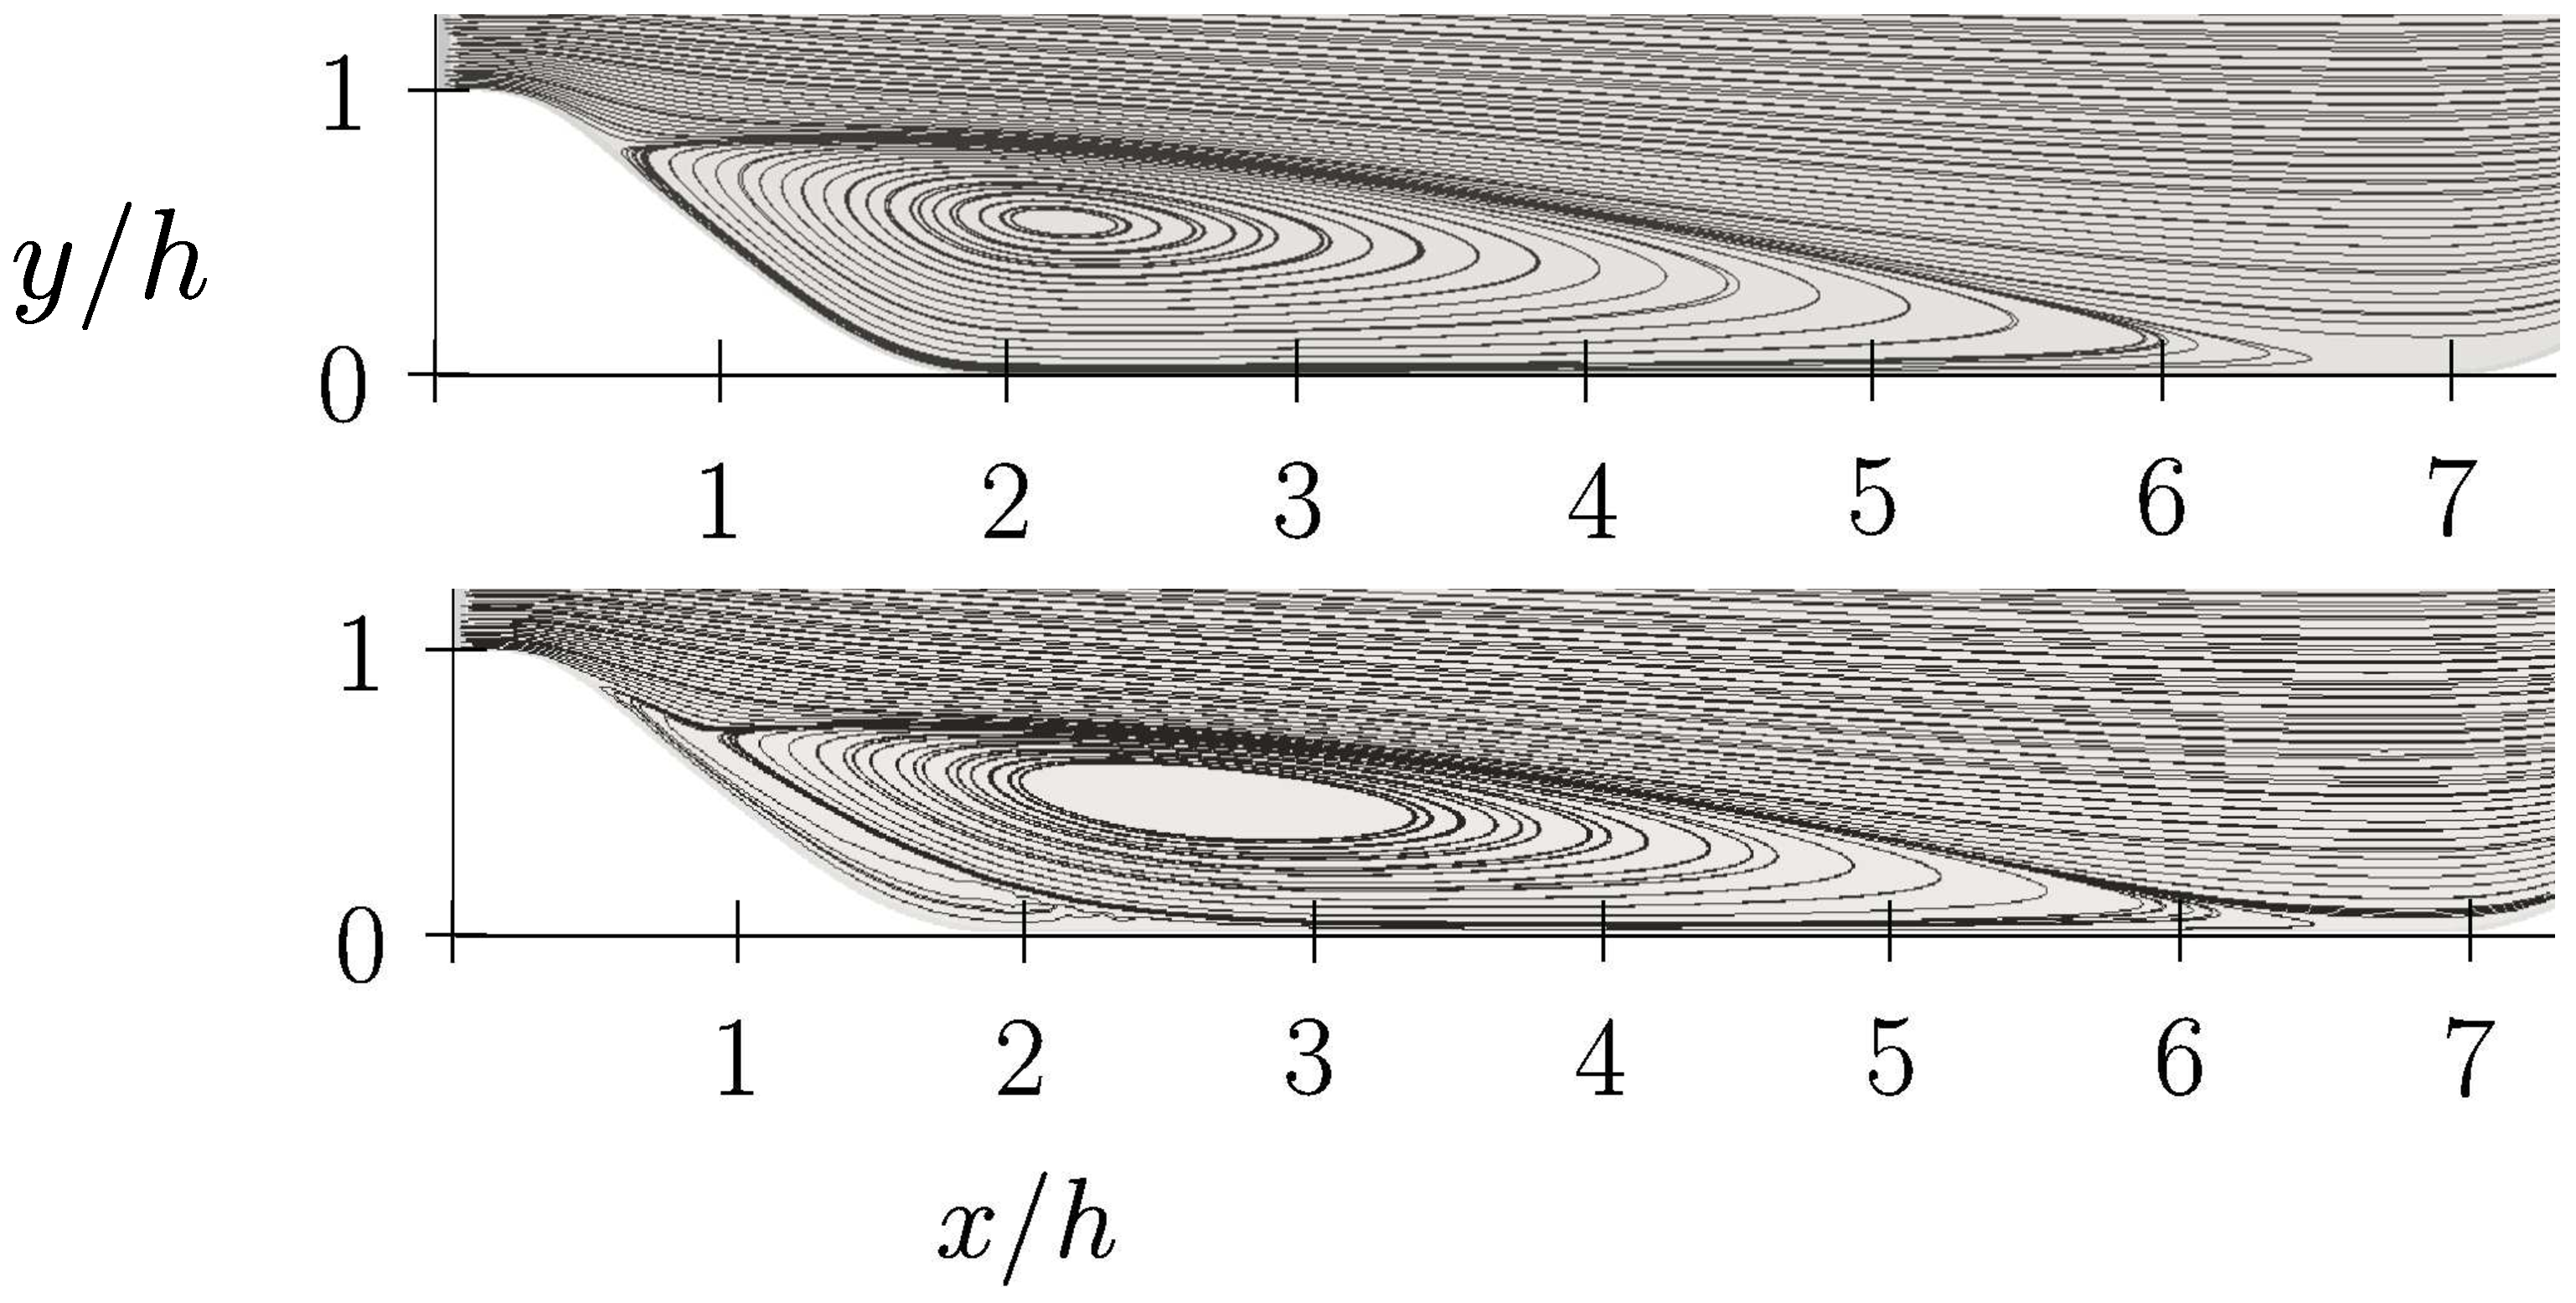
\includegraphics[width=1\linewidth]{chapter_5/figure/streamlines}
	\caption{Streamlines for the three cases tested. The top picture shows the case without the porous medium. The central picture shows the case where the porous media layer is put on the external part of the leeward side and the bottom case shows the case with porous medium put inside the leeward side.}
	\label{fig:streamlines}
\end{figure}


\begin{figure}[H]
	\centering
	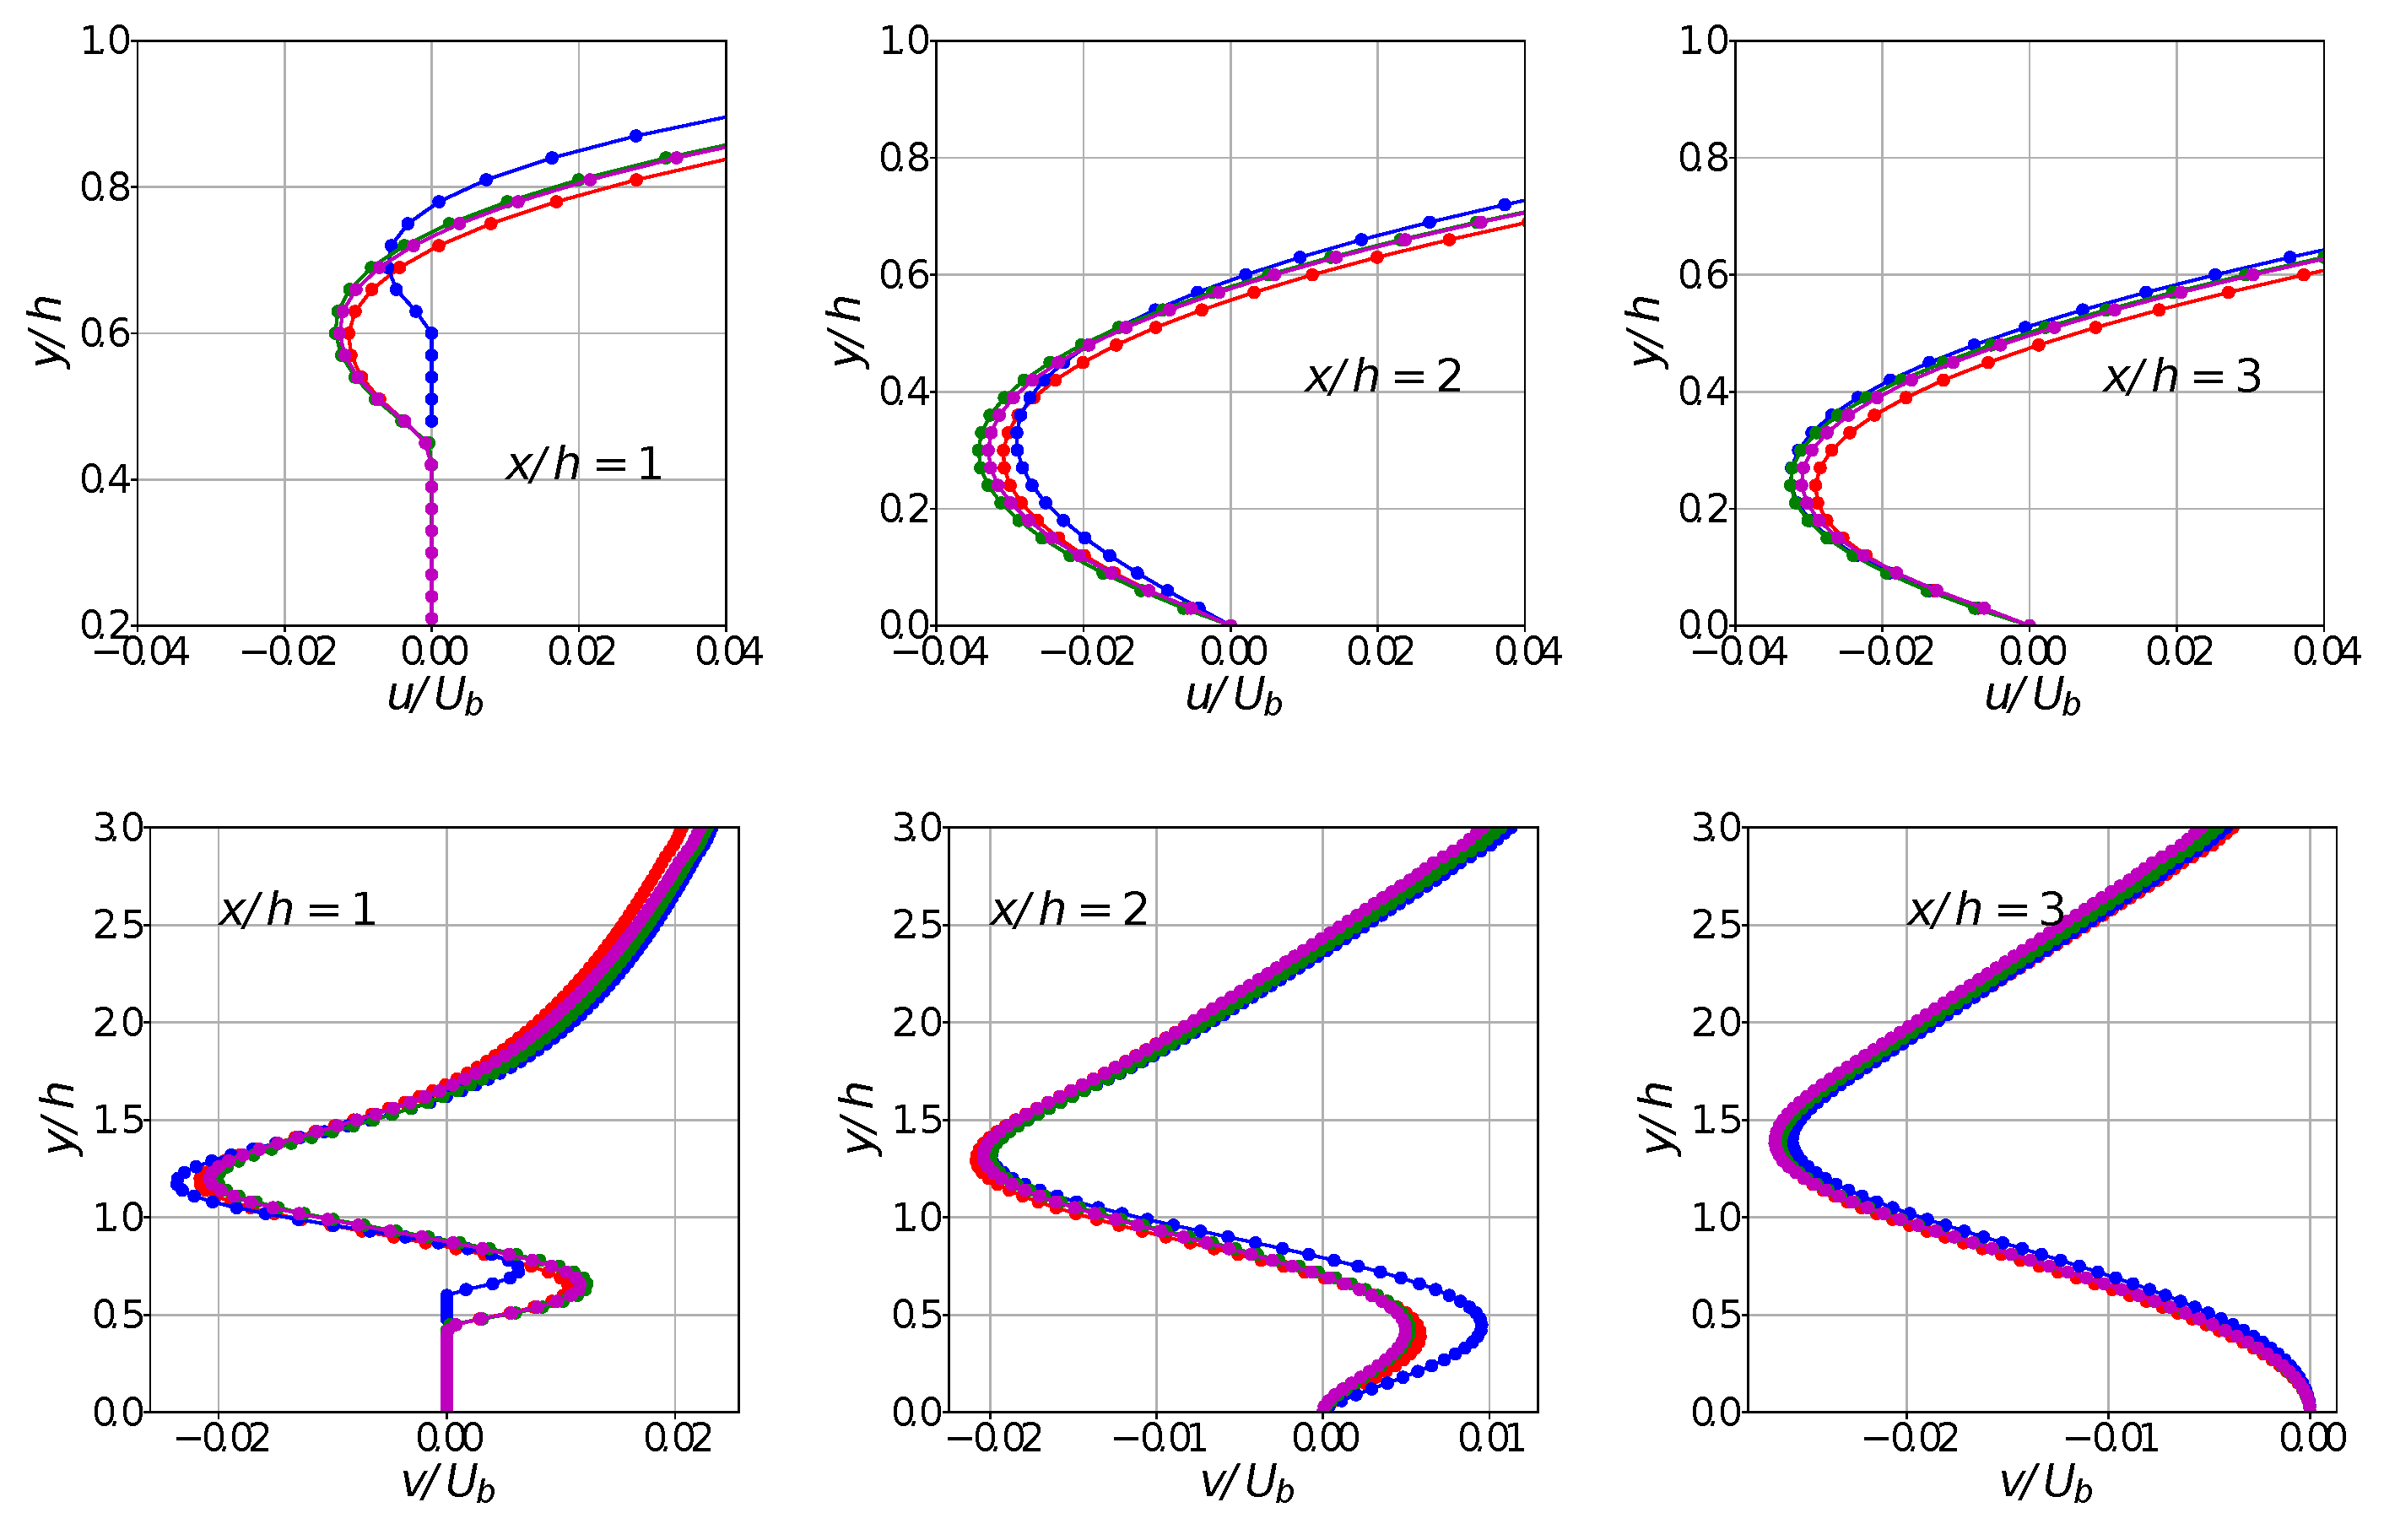
\includegraphics[width=1\linewidth]{chapter_5/figure/cuts_hill}
	\caption{The top three figures show the horizontal velocity profile for the sampled cut at $x=1$, $x=2$ and $x=3$ respectively from left to right. The bottom figures follow the same patterns but instead shows the vertical velocity profile. The red line is the \textbf{base} case the blue line is the \textbf{external case} and the green line is the \textbf{internal} case.}
	\label{fig:cuts_hill}
\end{figure}


\section{Conclusions}

In the chapter we have shown how the VANS equations derived in chapter 2 can be used to describe the averaged macroscopic field for rigid porous medium. We have also shown how the interface should be threated in order to retrieve good results. Direct comparison with DNS data show that the linear smoothing of the porosity field and of the effective permeability field are necessary. We have also shown that using the metamodel developed for $\mathbf{H}$ produces the same smoothing for the interface. Finally the periodic hill application demonstrate that our homogenized solver can be used easily as a tool to test and measure porous coating and their effectiveness.
For the porous characteristics used in our test we have found that the porous medium has negative effects for separation. But our focus was on the validation and easiness-to-use of our macroscopic model. With this tool it is now possible to extensively study porous media coatings in order to find the optimal characteristics for different objectives.
%If it would be possible to obtain systematically the same results with a reduced information model \footnote{like a general metamodel or a macroscopic model for porous media or a turbulence model for turbulent flow} and a full physic simulation we would be in a paradox. Basically it would means that some of the input information are redundant. This statements should be kept in mind when making analysis on the macroscopic model against the DNS.
